\documentclass[a4paper,twoside]{article}

%% Language and font encodings
\usepackage[spanish]{babel}
\usepackage[utf8]{inputenc}
\usepackage[T1]{fontenc}


%% Sets page size and margins
\usepackage[a4paper,top=3cm,bottom=2cm,left=2.5cm,right=2.5cm,marginparwidth=0.5cm]{geometry}

\usepackage{amsmath}			%Paquete matemático
\usepackage{graphicx}
\usepackage[colorinlistoftodos]{todonotes}

\usepackage{hyperref}		%Paquete empleado para colocar hipervinculos
\hypersetup{
 colorlinks = true,
 linkcolor = black,
}

\usepackage{eurosym}
\usepackage{pdfpages}			%Sirve para incluir PDF en el documento
\usepackage{anysize}			%Podremos colocar imagenes de cualquier tamaño
\usepackage{subfig}				%Nos permitira colocar varias imagenes en una figura
\usepackage{float}				%Podremos crear y colocar boxes donee queramos
\usepackage[export]{adjustbox}

%Colocamos cabeceras y pies de pagina
%(CONSULTA: http://edicionesoniricas.com/maquetar-latex-encabezados-pies-pagina/)
%(CONSULTA2: https://es.sharelatex.com/learn/Headers_and_footers)
%\bfseries es análogo a \textbf{}
% \leftmark-> Adds name and number of the current top-level structure (section for article) in uppercase letters.
%\rightmark-> Adds name and number of the current next to top-level structure (subsection for article) in uppercase letters.
\usepackage{fancyhdr}		%Paquetes necesarios
\pagestyle{fancy}			%Borra los parametros por defecto
\fancyhf{}
\fancyhead[RO,LE]{\bfseries\thepage}
\fancyhead[LO,RE]{\bfseries\rightmark}
%Nos aseguramos de que en las paginas plain, no haya ni cabeceras ni lineas
\fancypagestyle{plain}
{
 \fancyhead{} % elimina cabeceras en paginas "plain"
 \renewcommand{\headrulewidth}{0pt} % así como la raya
}

%Definimos las lineas divisoras de las cabeceras y pie de pagina
\renewcommand{\headrulewidth}{1pt}	%Define el grosor de la línea de head
\renewcommand{\footrulewidth}{0pt}		%Define el grosor de la linea foot (Si no queremos linea, 0pt)
\addtolength{\headheight}{0.5pt} % espacio para la raya

%Librerias para introducir código de Matlab
%\usepackage{bigfoot} % to allow verbatim in footnote
\usepackage[numbered,framed]{matlab-prettifier}
\lstset{
 style              = Matlab-editor,
 basicstyle         = \mlttfamily,
 escapechar         = ",
 mlshowsectionrules = true
}
\usepackage{listings}
\usepackage{xcolor} % for setting colors


% Pie de pagina
%\fancyfoot{} % limpia el pie
\fancyfoot[C]{- \thepage -} % número de página centrado

%Nos generará texto para pruebas de maquetado
\usepackage{lipsum}

% To include code in differents languages
%\usepackage{minted}
%\usemintedstyle{borland}
%\usepackage{mdframed}

% To can use multirow
\usepackage{multirow}
\usepackage{comment}
\usepackage{cite}
%----------------------------------------------------------------------------------------------------------------------------------
\begin{document}
\bibliographystyle{ieeetr}
\begin{titlepage}
\centering
\Huge{\textbf{AMPLIACIÓN DE ROBÓTICA}} \\
\Huge{Comparativa de técnicas de SLAM empleando un robot movil}\\

\vspace{1cm}
\LARGE{Grado en Ingeniería Electrónica, Mecatrónica y Robótica}\\
\rule{\textwidth}{0.1mm}
\large{\tableofcontents}
\vspace{1cm}
\rule{\textwidth}{0.1mm}
\Large{\textbf{Autores:} \\
                         López Gil, Miguel \\
                         Montes Grova, Marco Antonio\\
                         Osuna Cañas, Alfonso Carlos}
\end{titlepage}
\newpage

% %%%%%%%%%%%   INTRODUCCION %%%%%%%%%%%%%%%%%%
\section{Introducción al proyecto}
En este proyecto se implementan diferentes técnicas de SLAM visuales, así como diversas fuentes de odometría, sobre un robot móvil de bajo presupuesto.\par
El robot ha sido diseñado con una topología inspirada en los vehículos de exploración espacial conocidos como \textit{rovers}, utilizando materiales y métodos de construcción asequibles y manteniendo como objetivo una sencilla sustitución e iterabilidad de cada componente. La estructura está diseñada en FreeCad y compuesta por piezas de madera mecanizadas en una cortadora láser cnc. Algunos elementos sin funcionalidad estructural, como los encoders o el soporte de la cámara, han sido fabricados mediante impresión 3D.\\
La disposición geométrica es la de un vehículo diferencial, con tres pares de ruedas, cada una con su respectiva pareja de motor y encoder. Como drivers de los motores se han usado tres puentes H \textit{L293D} integrados en una placa de circuito impreso diseñada expresamente para ello.
\par
La odometría del robot se obtiene a partir de una estimación de la posición a partir de encoders ópticos, y de la velocidad y aceleración medidas por una IMU \textit{mpu-6050}. La fusión sensorial se realiza mediante un filtro de Kalman extendido, implementado en el paquete \textit{robot localization} de ROS kinetic. \\
Las imágenes y medidas de profundidad utilizadas para las técnicas SLAM provienen de una cámara \textit{Kinect for Xbox 360} de Microsoft, que cuenta con una cámara RGB y un sensor de profundidad matricial.

\newpage
\section{Hardware empleado en el proyecto}
Con el fin de obtener una vista general de todo el proyecto, así como del coste del mismo se lista a continuación todos los componentes del robot y su coste:
\begin{itemize}
	\item Chasis del vehículo. Fabricado a partir de un tablón plano de edf cortado en una cnc láser de forma gratuita gracias al Fablab de la Universidad de Sevilla en la facultad de Arquitectura.
	\item Motores de corriente continua(~1pavos). Adquiridos a través de tiendas digitales destinadas a la importación por un precio muy ajustado, tal y como se refleja en la calidad del producto. Sin embargo, formaban parte de un kit que incluye ruedas y acople al eje de transmisión, suponiendo un ahorro importante de tiempo y dinero. 
	\item Encoders ópticos (~6pavos). Compuestos por un diodo emisor de luz ()comprados también en los mismos sitios web que los motores) y por un disco que interrumpe el paso del haz lumínico diseñado específicamente e impreso en 3D.
	\item Microcontrolador ATmega328 (~10pavos). Aunque la gran parte del código implementado en el micro no utiliza las librerías de arduino, por comodidad se ha optado por un microchip ya montado en una placa tipo arduino (un modelo no oficial, clónico).
	\item IMU mpu-6050 (~2pavos).
	\item Raspberry Pi 3B+ (~30pavos). Constituye el cerebro del robot, y centraliza la comunicación con los demás sistemas. Aunque puede resultar el componente más caro del proyecto, se disponían de varias de antemano, por lo que no hubo que asumir su coste.
	\item Kinect for Xbox 360 de Microsoft (~15pavos). Esta popular cámara merece la fama que tiene por lo asequible que es (especialmente el modelo más antiguo) y las utilidades que trae. Se demuestra como la opción más socorrida para desarollar con poco presupuesto aplicaciones que requieran de imágenes o sensores de profundidad.
	
\end{itemize}
\subsection{Estructura}
El robot ha sido diseñado con una topología inspirada en los vehículos de exploración espacial conocidos como \textit{rovers}, utilizando materiales y métodos de construcción asequibles y manteniendo como objetivo una sencilla sustitución e iterabilidad de cada componente. La estructura está diseñada en \textit{FreeCad} y compuesta por piezas de madera mecanizadas en una cortadora láser cnc.
Algunos elementos sin funcionalidad estructural, como los encoders o el soporte de la cámara, han sido fabricados mediante impresión 3D. Todos los modelados pueden encontrarse en la sección hardware de GITHUB.
\begin{figure}[h!]
	\centering
	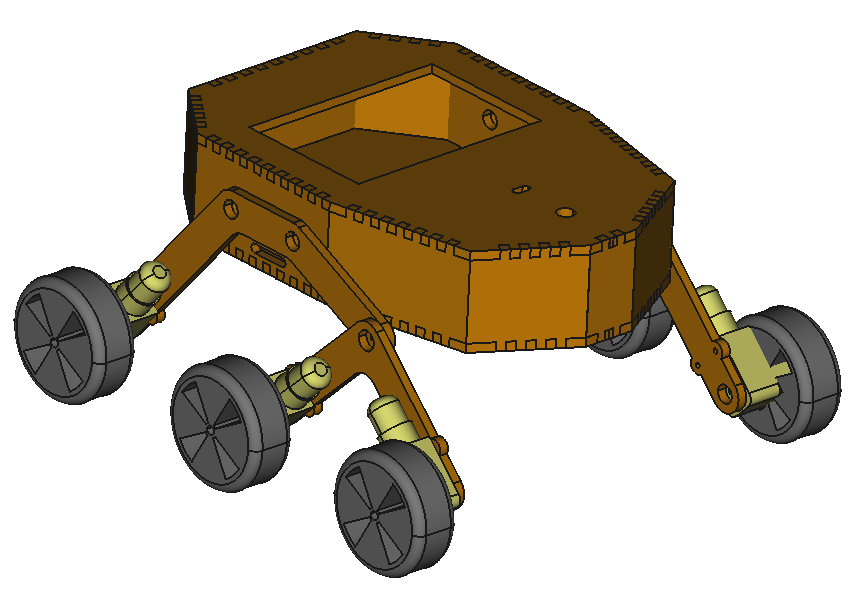
\includegraphics[width=.6\textwidth]{images/hw/wheele_stl}
	\caption{Modelo CAD del robot}
\end{figure}
\\
La disposición geométrica es la de un vehículo diferencial, con tres pares de ruedas, cada una con su respectiva pareja de motor y encoder.\\

\subsection{Motores DC}
 Los seis motores utilizados, a pesar de que deberían comportarse de forma parecida, presentan respuestas muy diferenciadas; para una señal de control idéntica cada uno de ellos muestran puntos de operación distintos y se observan respuestas ante escalón muy variadas. Sin embargo, todos presentan un comportamiento común, una gran zona muerta que complicará mucho la operación del robot a velocidades extremadamente bajas. En concreto, con el convesor digital-analógico del microcontrolador seleccionado (más detalles en la seccion2.arduino), se pierde un 40\% de los bits del rango de salida a causa de este incoveniente.  
 \begin{figure}[h!]
 	\centering
 	
\includegraphics[width=.6\textwidth]{images/hw/motor_est}
 	\caption{Característica estática de un motor}
 \end{figure}
\subsubsection{Especificaciones}
\begin{itemize}
	\item Tensión de trabajo: de (aproximadamente) tres a seis voltios.
	\item Corriente máxima: 120 miliamperios.
	\item Dimesiones: 70x22x18 milímetros.
	\item Reductora: 48 revoluciones a una.
	\item Peso (sin ruedas): 29 gramos.
\end{itemize}
\subsubsection{Drivers}
Debido a las bajas prestaciones y requerimientos de los motores, se ha optado por los drivers más asequibles disponibles: tres microchips L293D que integra cada uno dos puentes H. Como se explica más detenidamente en la seccion SOFEWARE, estos puentes H nos permiten configurar la dirección de giro con dos señales digitales y la velocidad con otras dos señales analógicas.\\
Por comodidad y robustez, se ha diseñado en \textit{KiCad} una placa de circuito impreso muy simple que facilita el cableado y permite integrar algún componente pasivo (como diodos fly-back o capacidades de by-pass). Gracias al laboratorio de electrónica este diseño ha sido revelado sobre una placa de una sola cara, obteniendo, como se aprecia en las imágenes, un acabado final bastante bueno.\\
 \begin{figure}[h!]
 	\centering
 	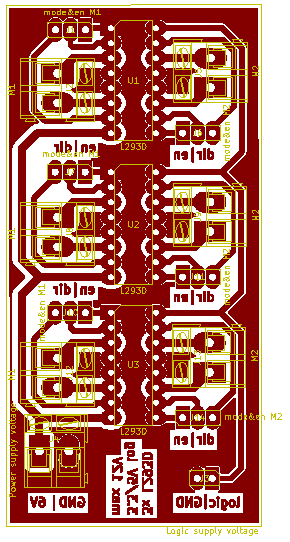
\includegraphics[width=.2\textwidth]{images/hw/pcb_kicad}
 	\caption{Diseño en KiCad de la PCB.}
 \end{figure}
  \begin{figure}[h!]
  	\centering
  	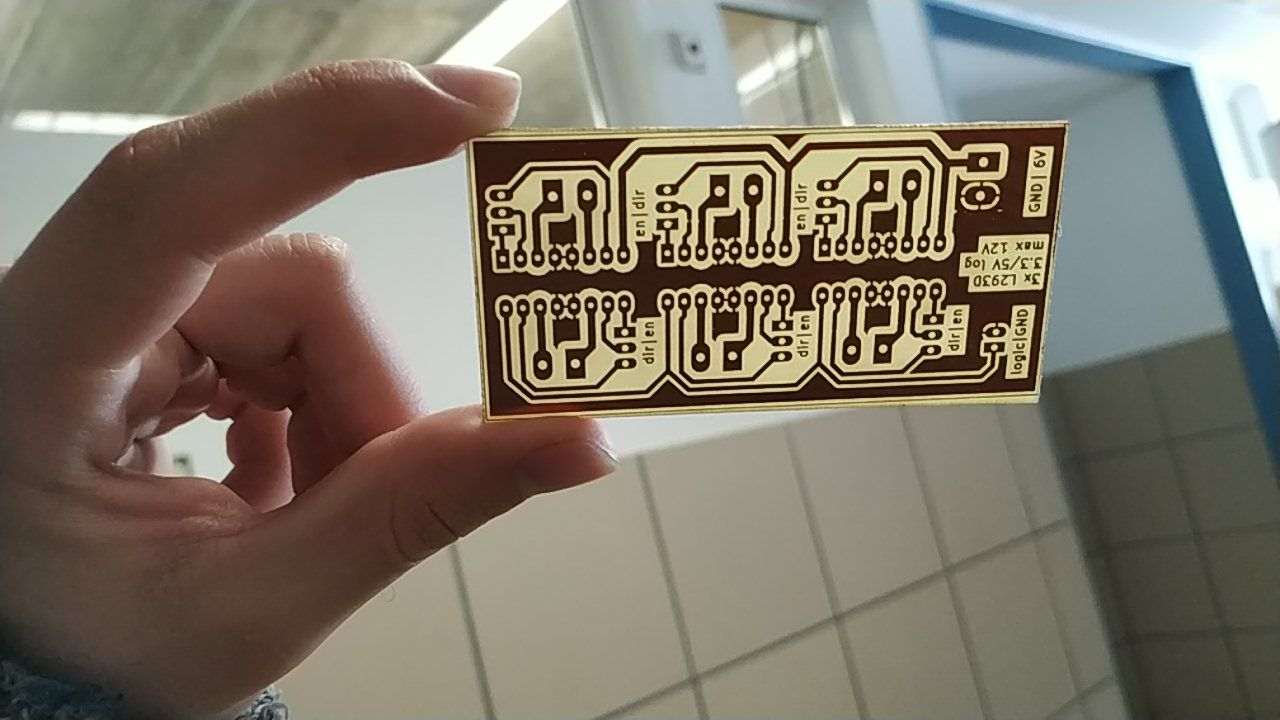
\includegraphics[width=.6\textwidth]{images/hw/pcb_img}
  	\caption{Acabado final de la PCB revelada.}
  \end{figure}
 Los microchips requieren de una referencia de tensión lógica (para operar la señal de entrada correctamente) y de una fuente de potencia capaz de alimentar los motores. La referencia se consigue de una salida de cinco voltios del arduino, que será quien se comunique con el driver. La alimentación de los motores corre a cargo de un transformador externo de 12V y XA.
	
<<<<<<< HEAD
\subsection{Encoders}
Los sensores elegidos para medir la velocidad de cada rueda y estimar la posición y velocidad del robot, son unos sencillos encoders ópticos binarios junto a unos discos perforados. Al pasar la luz por una perforación del disco, que gira a la misma velocidad que la rueda, se manda una señal digital al micro. Contabilizando los flancos de subida o de bajada en cierto periódo de tiempo, y conociendo las dimensiones del disco, se obtiene una estimación de la velocidad. Para más detalles en este proceso dirigirese a la ventanilla 3 seccion software encoders GRACIAS. \\
La corriente necesaria para que funcionen correctamente los encoders es mínima, por lo que se alimentan desde una salida de cinco voltios de baja potencia del arduino.
=======
\subsection{Encoders}\label{enc_hard}
Los sensores elegidos para medir la velocidad de cada rueda y estimar la posición y velocidad del robot, son unos sencillos encoders ópticos binarios junto a unos discos perforados. Al pasar la luz por una perforación del disco, que gira a la misma velocidad que la rueda, se manda una señal digital al micro. Contabilizando los flancos de subida o de bajada en cierto periódo de tiempo, y conociendo las dimensiones del disco, se obtiene una estimación de la velocidad. Para más detalles en este proceso dirigirese a la ventanilla 3 seccion software encoders GRACIAS. 
>>>>>>> 99be32a6af63629257e8615c8aa425785a982917
 \begin{figure}[h!]
 	\centering
 	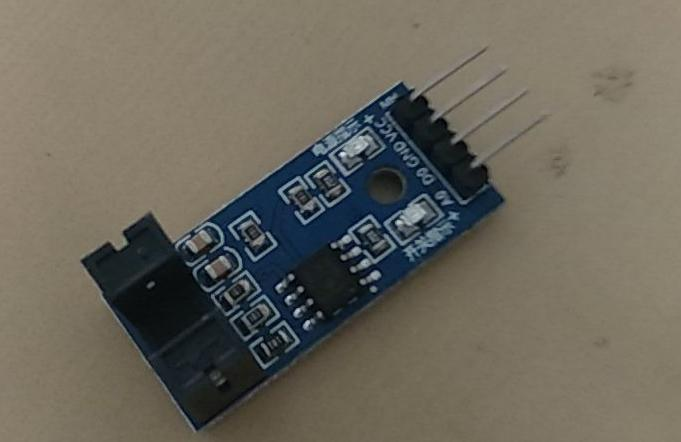
\includegraphics[width=.6\textwidth]{images/hw/encoder_img}
 	\caption{Encoder óptico. En negro resaltan el emisor y recepetor de luz.}
 \end{figure}
  \begin{figure}[h!]
  	\centering
  	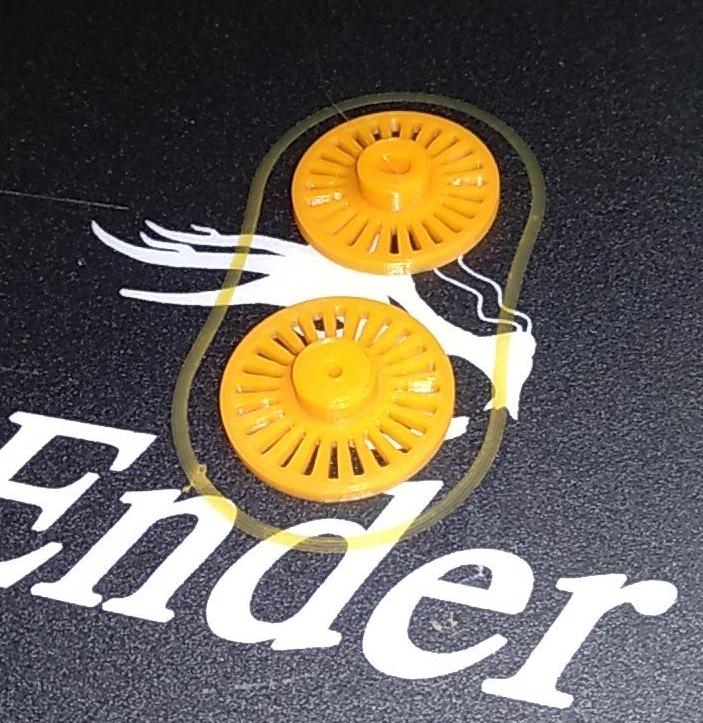
\includegraphics[width=.6\textwidth]{images/hw/encoder_stl}
  	\caption{Disco perforado impreso en 3D.}
  \end{figure}
  
\subsection{IMU}\label{imu_hardw}
Como ya se ha mencionado con anterioridad, se ha escogido una IMU mpu-6050 de seis grados de libertad para obtener datos de las velocidades y aceleraciones del robot. El microchip contine varios subsitemas, de los cuales nos interesa resaltar especialmente:
\begin{itemize}
	\item Giroscópio (tres ejes), con un rango progamable de ±250, ±500, ±1000 y ±2000 °/s (grados / segundos).
	\item Acelerómetro (tres ejes), con un rango progamable de ±2g, ±4g, ±8g y ±16g.
	\item Conversores analógico-digitales de 16 bits para las salidas del giroscópio y del acelerómetro.
	\item Bus i2c para ejecutar operaciones de lectura y escritura en cualquier registro del chip a una frecuencia máxima de 400kHz.
	\item Bus de comunicación auxiliar que posibilita introducir un magnetómetro en el futuro sin modificar el conexianado de todo el sistema.
\end{itemize}
Puesto que la IMU consume muy poca potencia en todo momento, se puede alimentar sin problemas desde cualquier salida de referencia de la Raspberry. 

\subsection{Ordenador de a bordo}
Debido a la multitud de entradas y salidas digitales y analógicas necesarias, al coste computacional de todo el sistema, y a la variedad de las comunicaciones, se plantea una configuración muy modular entre el ordenador de abordo (la \textit{Raspberry Pi}), los periféricos y la unidad de procesamiento para las partes más pesadas del software.\\
  \begin{figure}[h!]
  	\centering
  	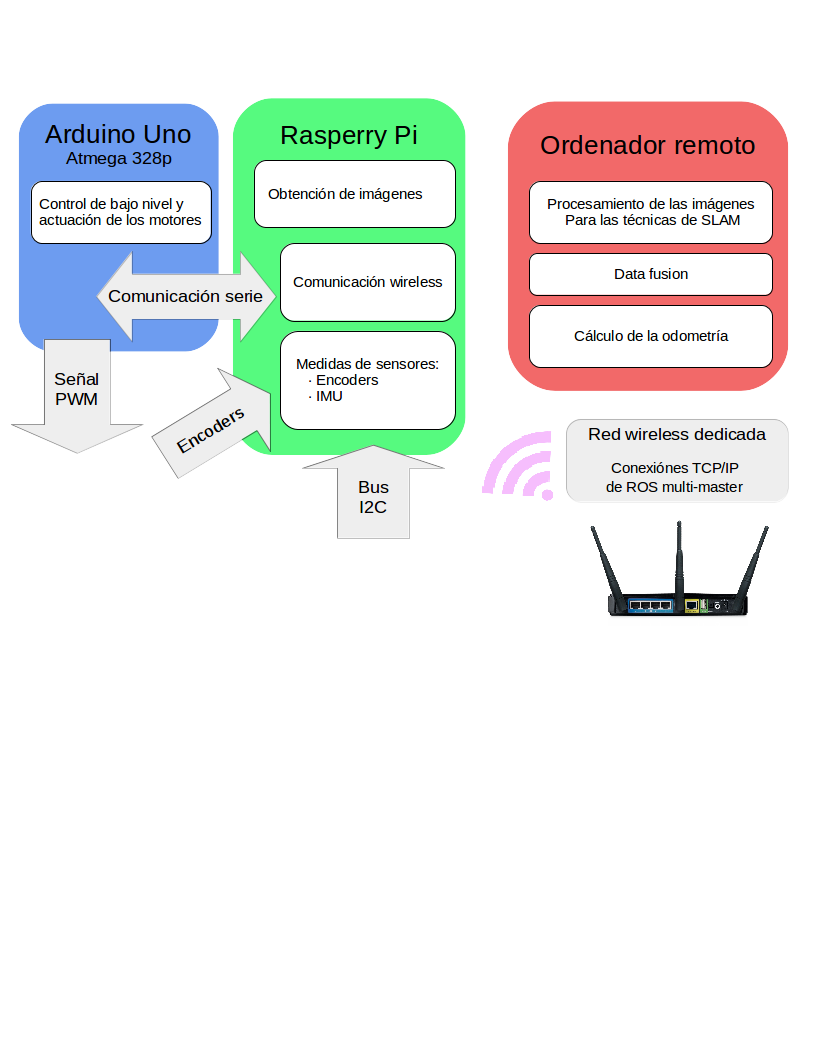
\includegraphics[width=.7\textwidth]{images/hw/wheele_esquema}
  	\caption{Esquema de conexionado de todos los componentes}
  \end{figure}\\
\subsubsection{Raspberry Pi}
Este \textit{single-boar computer}, como se le denomina en inglés, alberga muchas posibilidades. En el centro de todas ellas se encuentra un procesado ARM Cortex-A53 de 64-bit a 1.4Ghz capaz de correr varias distribuciones de GNU/linux. Con la limitada potencia gráfica de la que dispone, y su único gigabyte de memoria RAM resulta necesario procesar los cálculos más complejos en otro sistema más potente.\\
El modelo utilizado (3B+) incluye WiFi 802.11n a 150Mbit/s máximo. Sin embargo, es conveniente usar una antena WiFi externa más potente para conseguir más rango de señal.\\
La Raspberry es alimentada a través de un puerto micro USB a 5V con una corriente máxima de 2.5A aunque su lógica funciona a 3.3V.
\subsubsection{Arduino Uno}
Por conveniencia se ha optado por una placa arduino, que además de un microcontrolador ATmega328p, integra un puerto usb con un chipset que facilita su programación y la comunicación serie con el mismo. Incluye también un cristal de cuarzo , que provee una fuente prescisa para la señal de reloj y resulta especialmente útil para implementar el control de bajo nivel.\\
El micro cuenta con una memoria flash progamable de 32 kilobytes y una eeprom de un kilobyte, que es más que suficiente para el uso que se le va a dar. Dos timers de 8 bits y otro de 16 bits generan las interrumpciones necesarias para controlar el tiempo real e implementar el control. De todas las 23 posibles entradas/salidas digitales del micro, se ocupan cuatro salidas para seleccionar el sentido de la marcha de los motores (dos para todos las ruedas de la izquierda y dos para las de la derecha) y seis canales PWM para controlar la velocidad individual de cada uno.\\
La potencia eléctrica necesaria para que el micro, y sus periféricos, operen correctamente (5V y menos de 100mA) se obtienen por el puerto USB desde la Raspberry Pi, aprovechando el bus de comunicación serie.

\subsection{Cámara}
La \textit{Kinect for Xbox 360} integra una cámara RGB y un sensor de profundidad de luz infrarroja estructurada. El rango del sensor de profundidad alcanza, aproximadamente, de los 0.7 a los seis o siete metros. El campo de visión del dispositivo es de 57º horizontalmente y 43º en la vertical, aunque cuenta con un soporte motorizado capaz de inclinar la cámara MASMENOS 27º verticalmente. La resolución máxima de la cámara es de 1280x1024 píxeles, pero la más usada es 640x480 píxeles puesto que el frame rate depende fuertemente de la resolución con la que se trabaje, con un techo en los 30Hz.\\
La Kinect emplea un conector propietario que no es más que un conector USB con dos líneas de alimentación adicionales a 12 voltios.  
\subsection{Conexionado}

\newpage
\section{Software empleado en el proyecto}
\subsection{ROS}
ROS (Robotic Operating System) consite en un framework para la robótica sobre el que desarrolladores de cualquier 
ambito pueden aportar soluciones modulares a los sistemas de forma general. La modularidad de ROS hace que desarrollar 
un nuevo sistema o prototipo pueda ser una tarea tan sencilla como interconectar módulos de otros desarrolladores con 
los propios.\\
Esta característica lo hace idoneo para un proyecto como este en el que el uso de técnicas de percepción, 
mapeado, localization, etc, complejas se escapa del alcance; y solo sea necesario el desarrollo de modulos específicos de este robot
que sean capaces de comunicarse con aquellos más complejos y sean capaces de proporcionarle los datos necesarios para implementar los
algoritmos de SLAM. \\

El sistema operativo empleado tanto en el ordenador de abordo del robot,la Raspberry Pi, cómo en en el ordenador principal es Ubuntu 16.04, de tal modo que la distro de ROS en la que ha sido 
implementado el proyecto es ROS Kinetic Kame\footnote{https://wiki.ros.org/kinetic}.
\begin{figure}[!ht]
    \centering
    
\includegraphics[width=0.3\textwidth]{images/kinetic.png}
    \caption{Version de ROS empleada}
\end{figure}

\subsubsection{Interfaz con IMU}
Como ya se ha visto en la seccion \ref{imu_hardw}, al robot se le ha dotado con una IMU de 9 grados de libertad a fin de obtener medidas de aceleraciones.\\
La conexión se hace a través de una linea por protocolo $I^2C$, por lo que ha sido necesario el desarrollo de 2 `wrapers' en Python de funciones de bajo nivel; uno para el acceso a las
funciones de comunicación $I^2C$ a nivel de registros hardware y otro a nivel de funciones elementales para el manejo de los datos de la IMU.\\
Sobre ambos `wrapers' se ha escrito el nodo de ROS encargado de publicar los datos en 2 `topics', \textit{imu1\_rawImu} y \textit{imu1\_scaImu}, con los datos tal y como llegan 
de la IMU en el primero y reescalados en el segundo. El tipo de mensaje en el que se publican los datos es de tipo \textit{\href{http://docs.ros.org/kinetic/api/sensor_msgs/html/msg/Imu.html}{sensor\_msgs/Imu}}.\\

Como se trata de un sensor de bajo nivel que aporta información a los estratos más bajos del control, para poder disponer depués de mayor ancho de banda, se ha elegido una frecuencia de muestreo del sensor de $50\ [Hz]$; sufucientemente alta para no comprometer la estabildiad del sistema
 pero tambien lo sufucientemente baja como para no saturar el ordenador de abordo (teniendo en cuenta que este también deberá mantener un flujo constante de imagenes capturadas por la cámara, con el coste que eso conlleva).

 \newpage
 \subsubsection{Interfaz con encoders}\label{enc_soft}
Otro sensor añadido son los encoders mencionados en \ref{enc_hard}. Para su programación se ha desarrollado un `wraper' en C++ de la librería para Raspberr-Pi 3B \textit{pigpio} 
\cite{pigpio}. Como los encoders solo pueden ofrecer información de la magnitud de la velocidad y no del sentido es necesario hacer una conversión a nivel de sofware para poder
tener esa información.\\
Esto se hace suscribiendo el nodo creado al `topic' \textit{cmd\_vel}, de forma que de ahí se obtiene la referencia del sentido en el que se mueve el robot. Esta referencia se usa para reajustar el signo de las velocidades 
leidas directamente de los 6 encoders y publicarlas en el topic \textit{encoders} con el tipo de mensaje \textit{\href{http://docs.ros.org/jade/api/std_msgs/html/msg/Float64MultiArray.html}{std\_msgs/Float64MultiArray}}. La medida de los encoders, al tratarse de medidas de baja calidad con valores dispersos, han sido necesaria filtrarlas también.\\
En cuanto a la frecuencia de muestreo, se ha seguido la misma filosofia que con la programación del nodo de la IMU y se ha decido muestear a $50\ [Hz]$.

\subsubsection{Odometría}
A partir del calculo de la velocidad de las ruedas a partir de los encoders se desarrolló un nodo en ROS en el que se calcula la odometría del robot.\\
Para ello se han hecho una serie de suposiciones y simplificaciones del modelo del robot que después, en base a los resultados obtenidos, se han demostrado bastante acertadas.
\begin{itemize}
    \item Las ruedas tienen un modelo de rodadura perfecto y no deslizan en el suelo. Esto no es cierto en realidad y supone una fuente de errores importantes por la deriva que acumulan las posiciones estimadas, errores que son corregidos mediante una fusión sensorial.
    \item El modelo del robot consiste en un modelo diferencial de 2 ruedas. En base a esto a cada rueda `virtual' se le asigna el promedio de la velocidad de las 3 ruedas de cada bancada.
\end{itemize}
Las ecuaciones que definen el modelo del robot son las mostradas a continuación:
\begin{figure}[!ht]
    \centering
    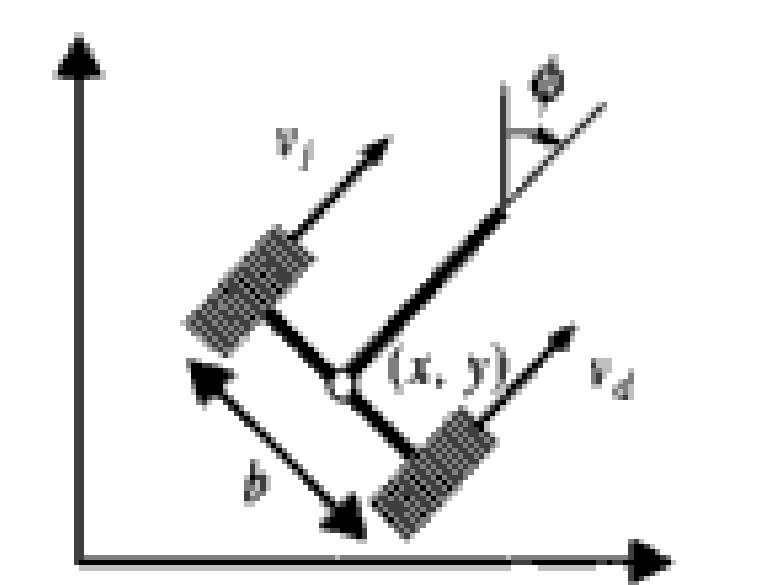
\includegraphics[width=0.3\textwidth]{images/dif_model}
    \caption{Representación posición y orientación modelo diferencial}
\end{figure}
\begin{center}
    $v=\dfrac{v_{dcha}+v_{izqd}}{2}$ \hspace{2cm} $\theta=\dfrac{v_{dcha}-v_{izqd}}{b}$
\end{center}
dónde \textit{v} es la velocidad lineal, \textit{w} la velocidad angular y \textit{b} la distancia entre las ruedas.\\
Y se definirá la posición y la orientación del robot cómo:
\begin{equation}
    \begin{pmatrix}
        \dot{x} \\
        \dot{y} \\
        \dot{\theta}
    \end{pmatrix}=
    \begin{pmatrix}
        cos(\phi) & 0 \\
        sin(\phi) & 0 \\
        0 & 1 \\
    \end{pmatrix}
    \begin{pmatrix}
        v \\
        \theta
    \end{pmatrix}
\end{equation}
Este nodo se suscribe al desarrollado en \ref{enc_soft} en el `topic' \textit{encoders}, y cada vez que llega un mensaje nuevo con los datos de los 
encoders calcula el avance del robot en base al modelo propuesto. La publicación de los datos se hace en el `topic' \textit{odom} a un ratio de $25\ [Hz]$ 
con un mensaje del tipo \textit{\href{http://docs.ros.org/kinetic/api/nav_msgs/html/msg/Odometry.html}{nav\_msgs/Odometry}}.

\subsubsection{Interfaz Raspberry-Pi/Arduino}
La comunicación por puerto serie se implementa haciendo uso de la librería \textit{CmdMessenger}. MIGUEL LAS PUTAS REFERENCIAS ACUÉRDATE., que permite definir comandos (con la posibilidad de asociarles argumentos y callbacks) de forma eficiente y sencilla.
Por la parte de la Raspberry, se usan las librerías CmdMessenger (escrita en c) o su alternativa PyCmdMessenger (en Python) en el nodo serial\_com.py para transmitir por el puerto serie.\\
Los siguientes comandos son los más importantes \\
Cmd\_off; Al recibir este comando el micro pasa a no hacer nada, comportándose como un apagado de emergencia. \par
De esta forma es sencillo publicar un tópico de 'comandos del sistema', como apagar o funciones de debugeo, y otros tópicos para los datos que hayan de retransmitirse. Cuando llegan datos desde el arduino, se ejecuta un callback (de la librería externa, no de ROS) que publica dicha información el tópico correspondiente. Si es el caso contrario, y se busca enviar datos al arduino, el nodo se subscribirá al tópico con ese dato y en el callback asociado (ahora sí de ROS) se envía al arduino.

\subsubsection{Interfaz Arduino/Motores}
Same old same old

\subsubsection{Computación distribuida con ROS-Multimaster Package}
Las técnicas de SLAM a testear en el robot desarrollado son computacionalmente costosas. Todo este coste computacional es
imposible asumirlo desde una Raspberry-Pi, por lo que surge la necesidad de hacer el procesado en un servidor remoto al robot en tiempo real con las 
dificultades que eso conlleva, entre ellas y la mas importante, la sincronización de datos.\\
Bajo estas condiciones de diseño y restricciones aparece una solución de la comunidad: ROS multimaster\_fkie. La premisa que lo rige es simple, dado un sistema mutirobot
cada elemento mantiene la ejecución de 2 nodos locales, \textit{master\_discovery} y \textit{master\_sync}; el primero es el encargado de mantener una lista del resto 
de \textit{roscores} disponibles en la red y de publicar el suyo propio como activo. El otro es el encargado de suscribir su \textit{core} los nodos de otros \textit{cores}.\\
Des esta forma todos tienen acceso de una forma hasta cierto punto `real-time' a los recursos del resto. 
\begin{figure}[!ht]
    \centering
    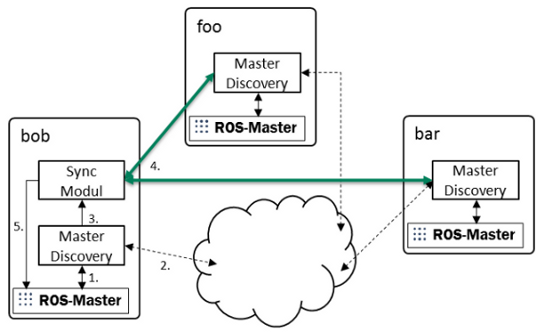
\includegraphics[width=0.6\textwidth]{images/ros_multimaster.png}
    \caption{Esquema del funncionamiento básico del paquete Multimaster}
\end{figure}
En este proyecto su integración se ha llevado a cabo lanzando en la Raspberry-Pi y en otro PC los nodos correspondientes siendo la Raspberry-Pi la 
suministradora de información y el PC el encargado de procesarla.
\subsection{Implementación filtro estadístico}
Introducción de porqué es interesante y eso, lo de vender la moto as usual
\subsubsection{Filtro de Kalman Extendido}
Background teorico que coma espacio, poner la imagen del filtro esa con colores bonicos y eso
\subsection{Implementación de filtro estadístico}
La información que el sistema obtiene de los sensores está sujeta a ruido e incertidumbres de la medida. A fin de minimizar los errores y mejorar la estimación de la posicion y velocidad del robot se ha 
considerado que era de especial interes y utilidad la aplicación de un filtro recursivo Bayesiano como estimador de estados, en concreto el filtro de Kalman extendido.
\subsubsection{ROS-Robot Localization Package}

\subsection{Arquitectura general del sistema}
Aqui lo de rqt\_plot and eso
\begin{figure}[!ht]
    \centering
    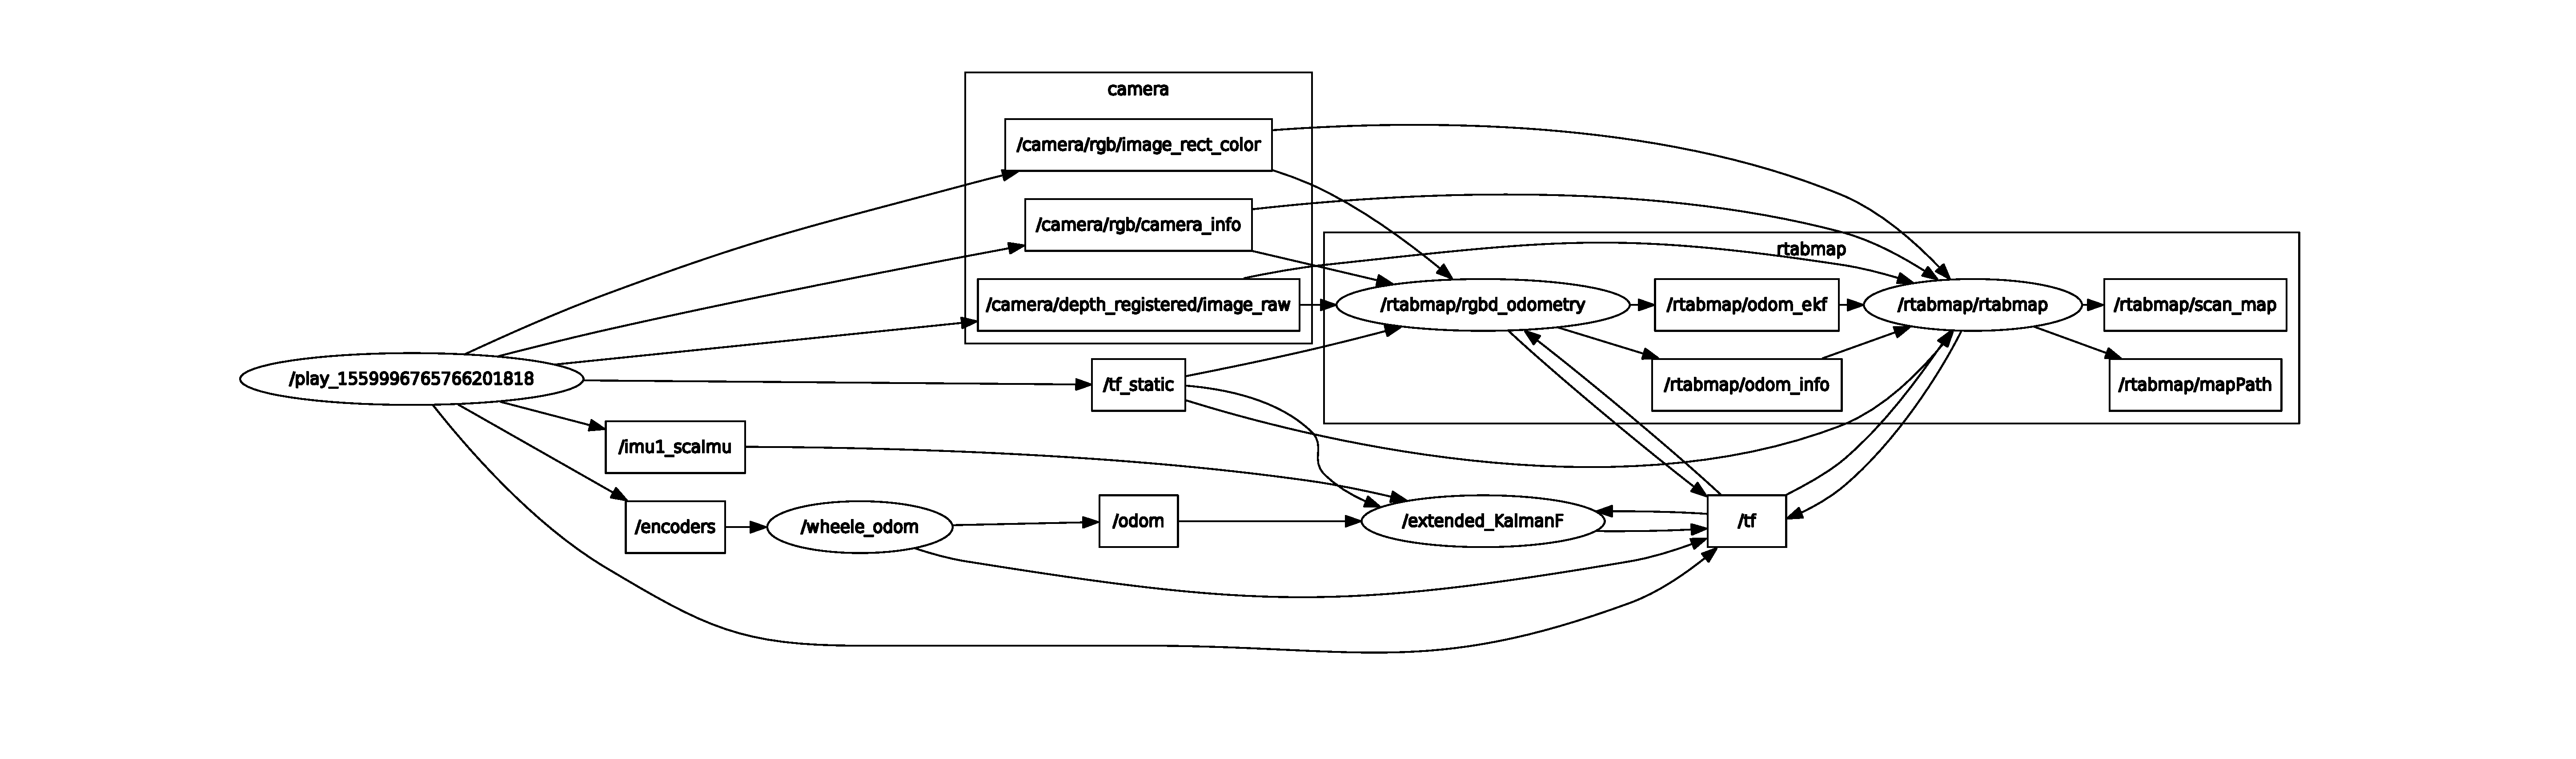
\includegraphics[width=\textwidth]{images/rqt_graphs/graph_RTABMAP.pdf}
    \caption{Captura de los nodos ejecutandose durante uno de los experimentos realizados con el robot}
    \label{rqt01}
\section{Puntos destacables de la implementación del proyecto}
\subsection{Obtención de los parámetros de la cámara}
Destacar que, siempre es necesario conocer los parámetros intrinsecos de la cámara además de la matriz de rotación. \\
Para obtener la matriz de parámetros de nuestra cámara, se ha hecho uso del paquete de ROS, \textit{\href{http://wiki.ros.org/camera_calibration}{Camera\_calibration}}.\\
Este paquete nos proporcionará la herramienta mostrada a continuación, que gracias a un tablero de ajedrez nos dará los parámetros intrínsecos de nuestra cámara:
\begin{figure}[!ht]
    \centering
    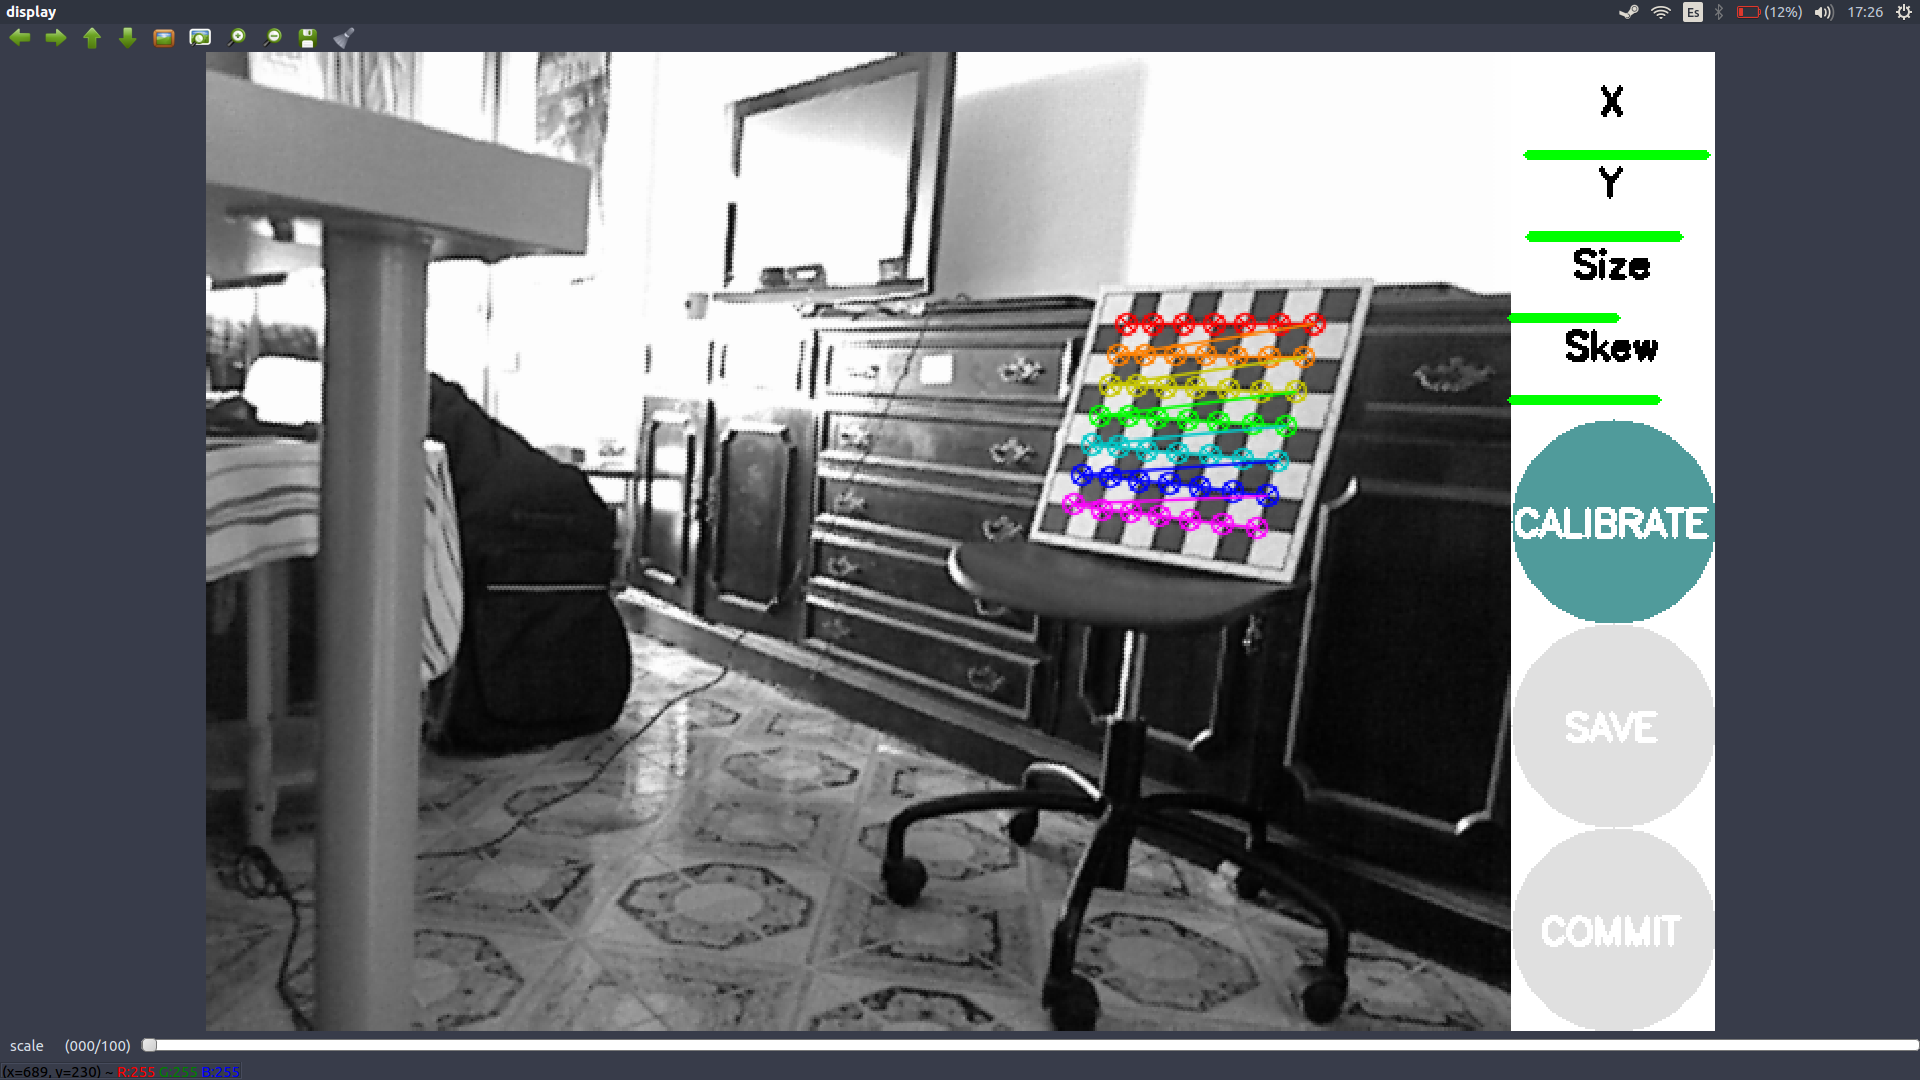
\includegraphics[width=0.8\textwidth]{images/calibration_art}
    \caption{GUI proporcionada por el paquete}
\end{figure}

Las matrices serán dadas en pormato \textit{.ost} y \textit{.yaml} que, despues se le pasará cuando se quiera emplear la cámara para actualizar el topic camera\_info,cuyo 
tipo de mensaje será \textit{\href{http://docs.ros.org/melodic/api/sensor_msgs/html/msg/CameraInfo.html}{sensor\_msgs/CameraInfo}}.\\

\newpage
\subsection{Inicialización del robot}
Para lanzar todos los nodos de ROS en el ordenador de abordo del robot y en el ordenador principal se han creado los siguientes ficheros \textit{roslaunch}:
    \begin{figure}[!ht]
        \centering
        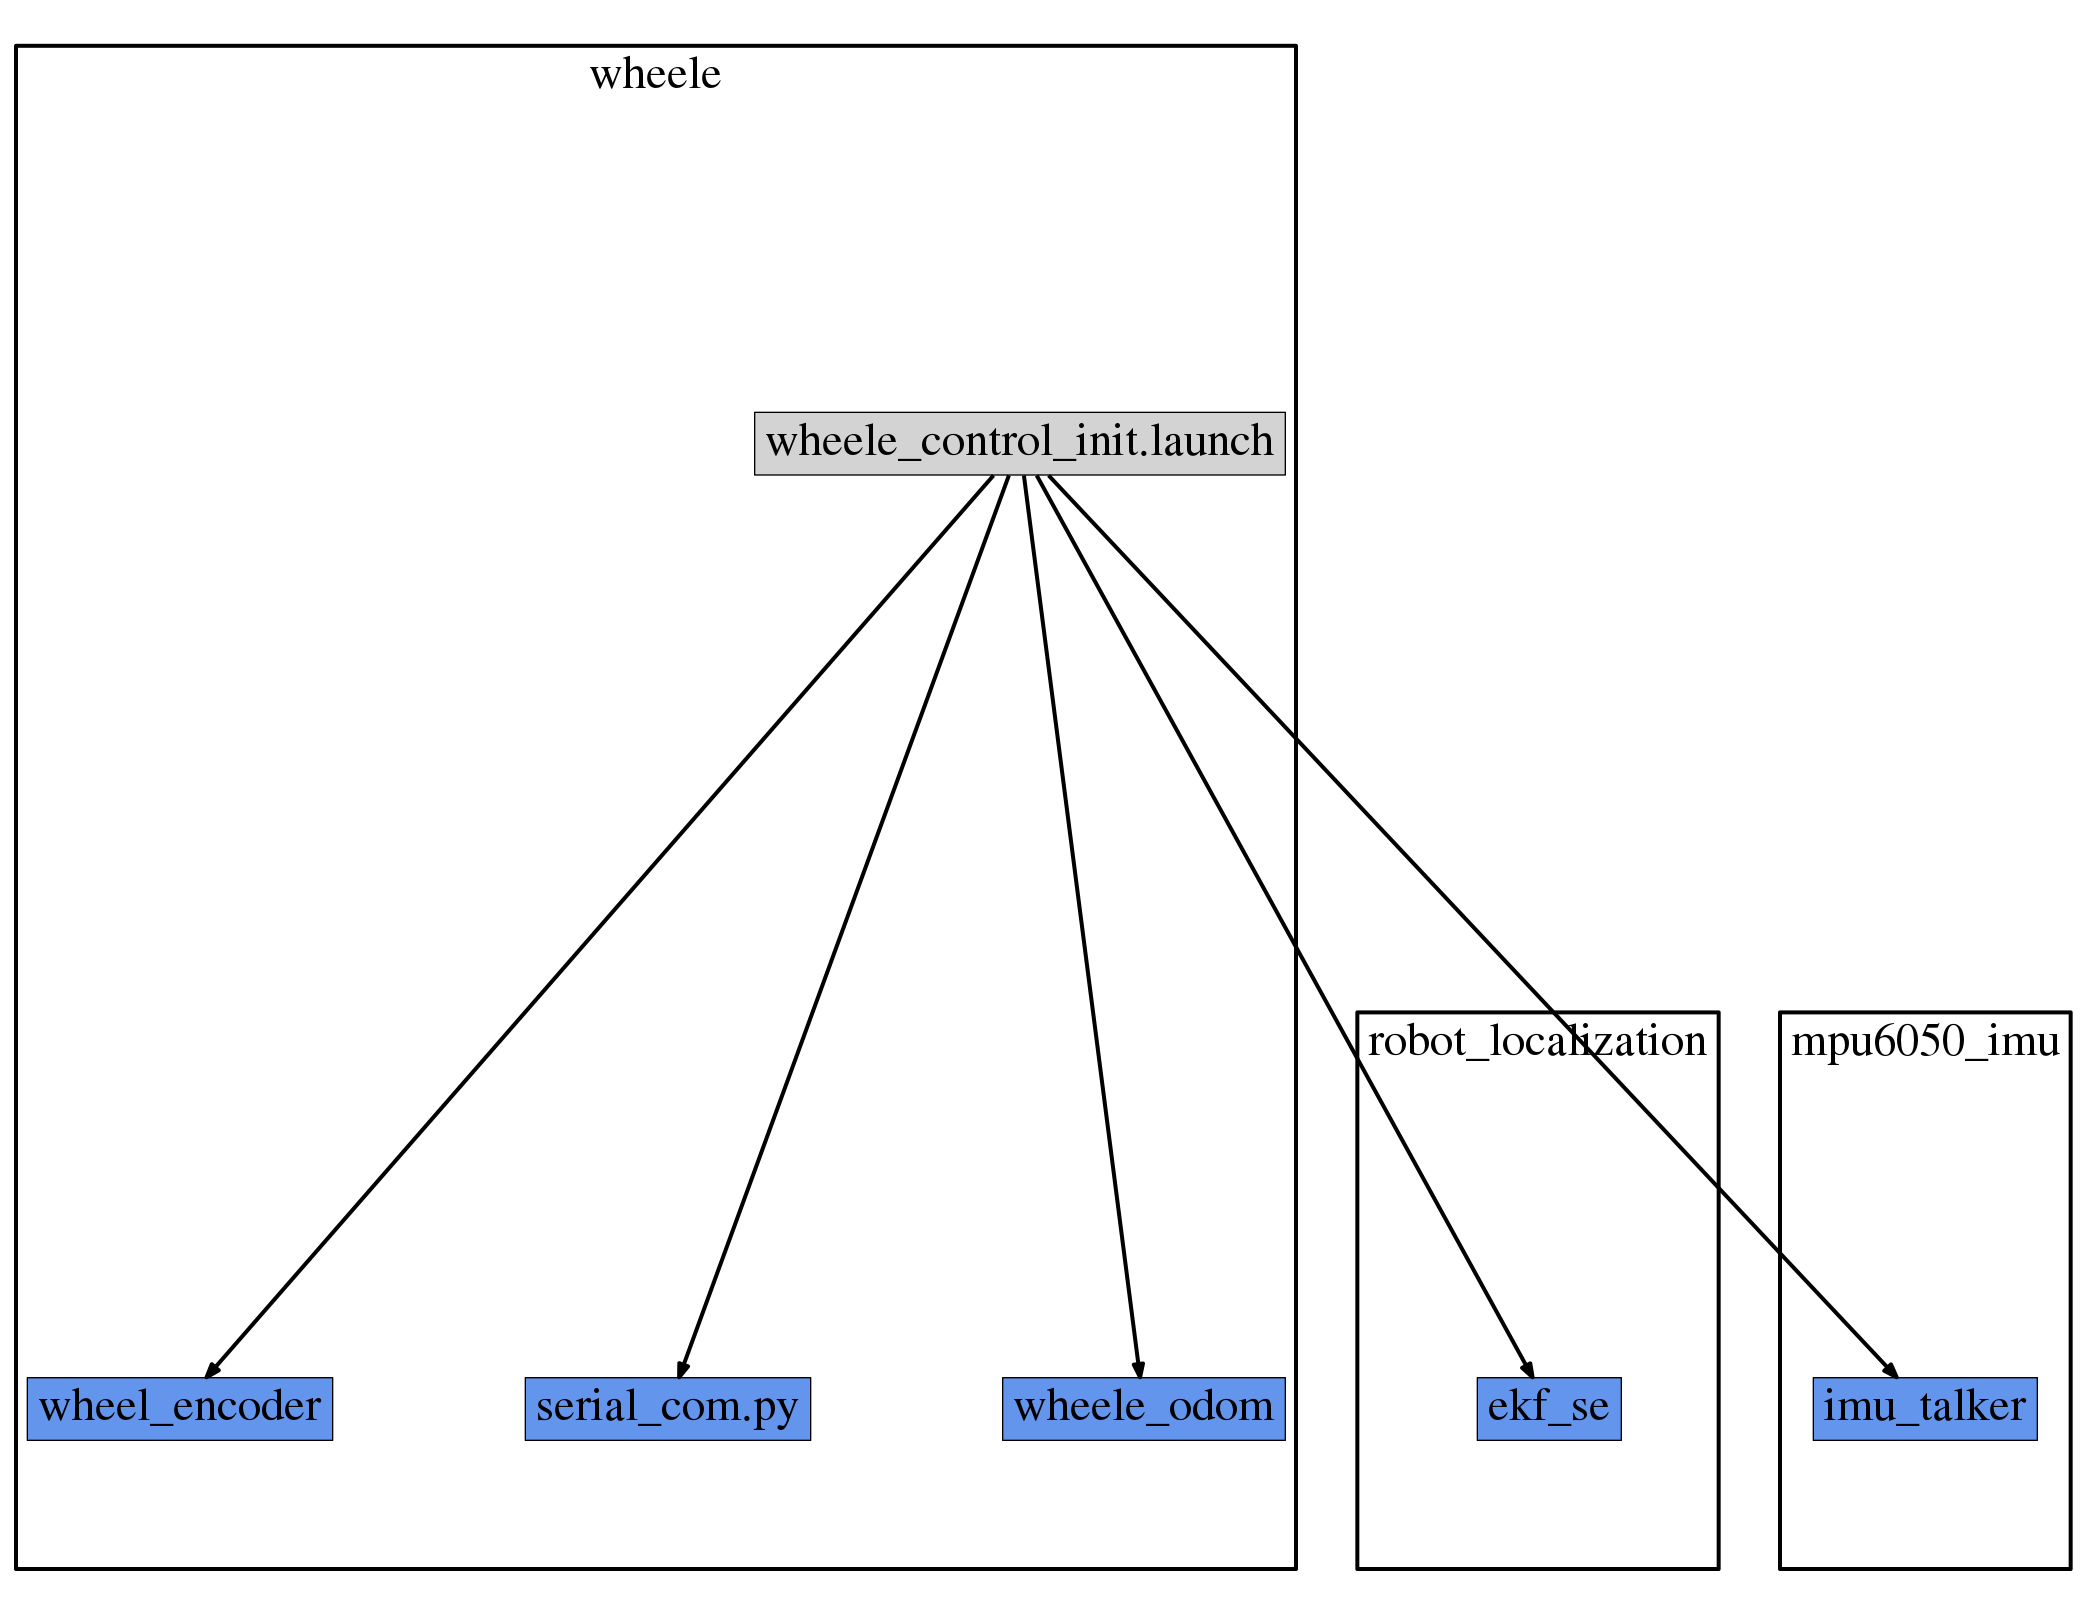
\includegraphics[width=0.6\textwidth]{images/whee}
        \caption{Nodos lanzados en el robot}
    \end{figure}

También se lanzarán los drivers de la cámara, aunque no aparezcan en la imagen. Los drivers son proporcionados por el 
paquete de ROS \textit{\href{https://github.com/ros-drivers/freenect\_stack}{Freenect}}.
Para poder tener control del motor integrado en la cámara, se ha empleado el paquete \textit{\href{https://github.com/muhrix/kinect_aux}{Kinect-aux}}.
    

\end{figure}


\newpage
\section{Análisis e introducción a las técnicas de SLAM}
El SLAM\textit{(Simultaneous Localization and Mapping)} es una tecnica cuyo objetivo es contruir un mapa de un entorno desconocido con un robot movil 
y conocer la posición de dicho robot dentro del mapa. \\
El primer planteamiento de la resolución de estos dos problemas cómo son la localización de un robot y la creación de mapas de manera conjunta surgió 
en 1986 en un congreso del IEEE en San Francisco. \\
Durante aquellos años, se habia comenzado a introducir métodos probabilistico en la inteligencia artificial 
y en la robotica. En dicha conferencia, se llegó a la conclusión de que la generación de mapas consistentes y localización de manera probabilistica era
un problema fundamental.\\

Tras ello, se establecieron las bases estadisticas para describir la relaciones entre \textit{landmarks}, objetos de referencia y 
para manipular la incertidumbre geométrica. \\
El planteamiento básico del problema de SLAM es el mostrado a continuación:
\begin{figure}[h!]
    \centering
    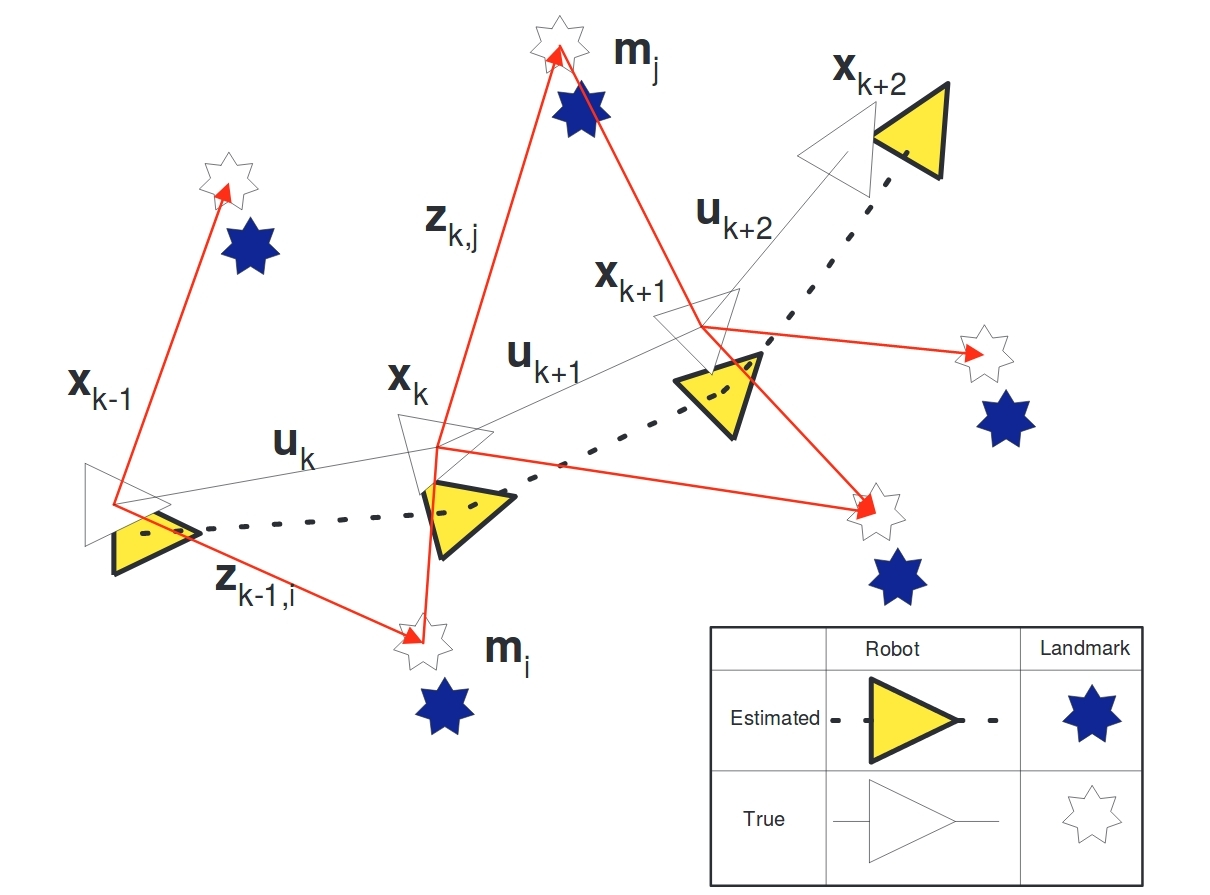
\includegraphics[width=.6\textwidth]{images/slam_prob}
    \caption{problema básico de SLAM}
\end{figure}

Dado un robot que se mueve por un entorno desconocido tomando observaciones relativas de un número desconocido de landmarks empleando un sensor posicionado
en el robot. Para el instante \textit{k}, se definen las siguientes variables:
\begin{itemize}
    \item $\textbf{x}_k$: Vector de estados que describe la posición y orientación del vehículo.
    \item $\textbf{u}_k$: Vector de control aplicado el instante anterior sobre el vehículo para que se encuentre
en el estado $\textit{x}_k$ en el instante \textit{k}.
    \item $\textbf{m}_i$:Vector que describe posición del i-ésimo landmark cuya verdadera ubicación se supone invariable con el tiempo.
    \item $\textbf{z}_{ik}$: Observación tomada desde el vehiculo de la posición del i-ésimo landmark en el instante \textit{k}.
\end{itemize}
Por tanto, se deberá computar la siguiente distribución probabilistica en cada instante \textit{k}:
\begin{equation}
    P\Big( \textbf{x}_k ,m | \textbf{Z}_{0:k},\textbf{U}_{0:k},x_0\Big)
\end{equation}
La solución se obtendrá de manera recursiva empleando el teorema de Bayes en un proceso en dos pasos: \textit{Time-Update} y \textit{Measurement-Update}. Para ello,
será necesario conocer el modelo de observación y el de movimiento. \\
A continuación se mostrará el modelo de observación y movimiento respectivamente:
\begin{center}
    $P\Big( \textbf{z}_k | \textbf{x}_{k},m \Big)$ \hspace{2cm} $P\Big( \textbf{x}_k | \textbf{x}_{k-1},\textbf{u}_{k} \Big)$
\end{center}

Una vez planteado de manera superficial el problema a resolver, el modo de abordarlo se ha desarrollado en muchas direcciones durante los últimos 20 años. \\
Algunos de estos métodos se muestran a continuación y se hablará de ellos, para posteriormente indagar en dos técnicas concretas.
\subsection{Clasificación técnicas de SLAM}
La forma en que se toma información de las imagenes que recibe y de su entorno y cómo la procesa permite distinguir las siguientes tipos de sistemas
SLAM visual:
\begin{itemize}
\item \textit{Denso vs Disperso} \\
En función de la cantidad de datos tomada de cada imagen, se realizará ésta clasificación. Las técnicas de SLAM disperso sólo emplean una pequeña
región de pixeles, cómo pueden ser puntos característicos. Sin embargo, las técnicas densas emplean la mayoría o todos los píxeles de cada frame
que reciben. \\
Debido a que la cantidad y tipo de información que toman son diferentes, el tipo de mapa que se obtendrá también lo es. Con las técnicas de SLAM
disperso se obtendrá una nube de puntos que será una representación de los puntos característicos de las escena y se usará sobre todo para hacer
un tracking de la pose de la cámara. Por otro lado, un mapa denso tendrá muchos más detalles y, requerirá de una mucho más elevada carga computacional.

 \item \textit{Directo vs Indirecto} \\
En función de cómo las técnicas de SLAM empleen y traten la información que reciben, se podrá clasificar en SLAM directo o indirecto.\\
El SLAM Indirecto, se basa en extraer primero las features de la imagen, puntos característicos, para posteriormente emplearlos para localizarse y contruir
el mapa. Para extraer estos puntos caracteristicos existen muchos descriptores: ORB, SIFT, FAST, etc. \\
En contraste, el SLAM Directo,emplean directamente la intensidad de los pixeles, de tal modo que se obtengan features intermedios. Estos metodos tratan de 
obtener la profundidad y estructura del entorno a partir de una optimización del mapa. Los procesos de extracción de puntos característicos son mucho más
pesados computacionalmente si se trabaja al mismo rate que un slam indirecto.\\
Por último, destacar, que los metodos indirectos de SLAM son más tolerantes a los cambios de iluminación del entorno.\\

A continuación, se monstarán una comparativa de una serie de técnicas de SLAM:
\begin{figure}[h!]
    \centering
    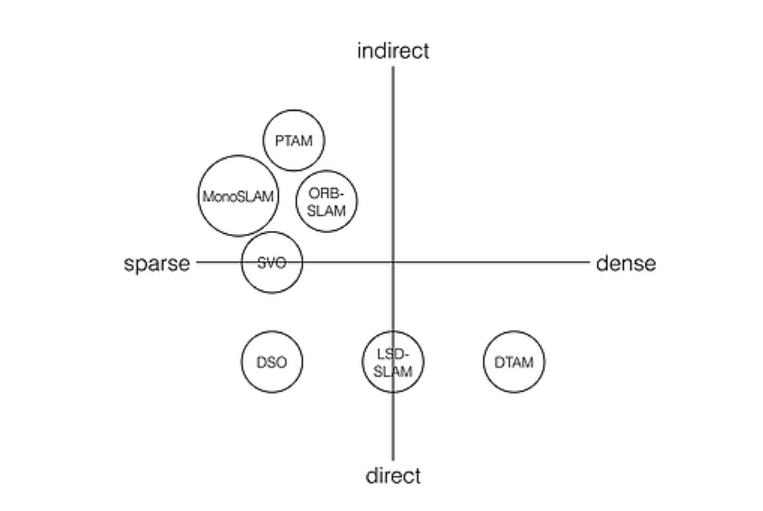
\includegraphics[width=.6\textwidth]{images/comp_slam}
    \caption{Comparativa de técnicas SLAM}
\end{figure}

\end{itemize}

\subsection{Técnicas SLAM implementadas en éste proyecto}
Destacar que, mientras la primera técnica de SLAM es una técnica determinista, la segunda será probabilistica.
\subsubsection{\textit{RTAB-Map SLAM}}
RTAB-Map \textit{(Real-Time Appearance-Based Mapping)} es una técnica de Graph-SLAM\footnote{http://robots.stanford.edu/papers/thrun.graphslam.pdf} basada en la detección de bucles cerrados incrementales. Es totalmente funcional 
con sensores RGB-D, Stereo y LIDAR. \\
El detector de bucles cerrados se basará en la comparativa de cuán semenjantes son la imagenes en una localización y la previa. Cuándo una hipótesis 
de bucle cerrado es aceptada, se añade una nueva restricción al \textit{graph} del mapa y, tras ello, el optimizador minimiza el error del mapa. \\

\begin{figure}[h!]
    \centering
    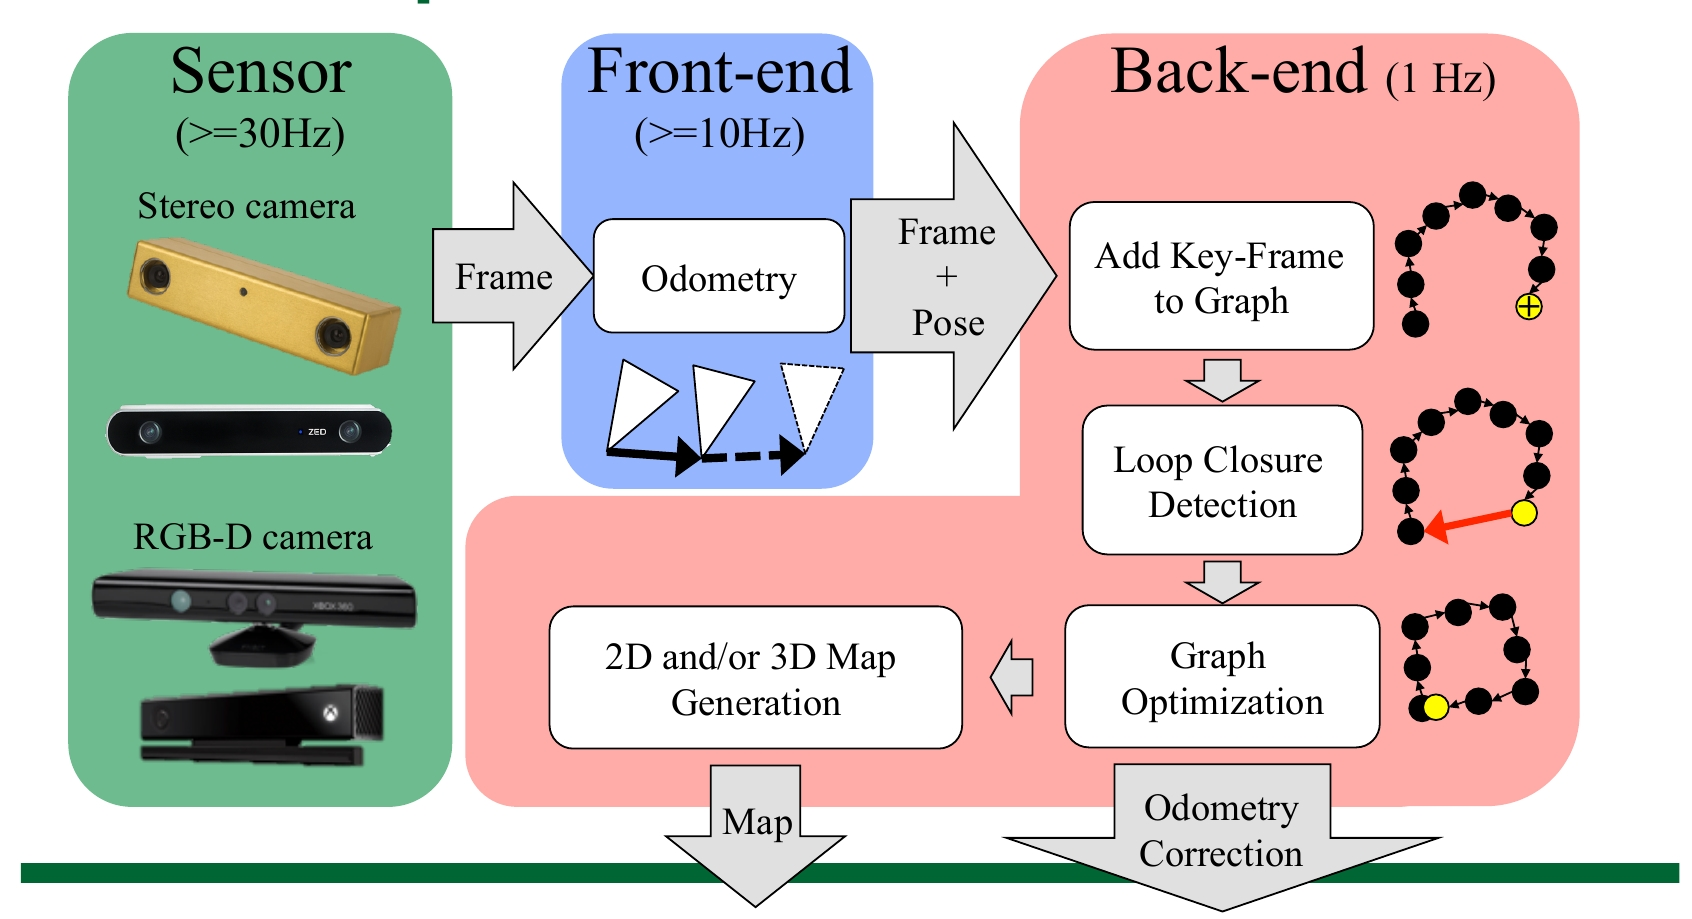
\includegraphics[width=.7\textwidth]{images/rtabmap_scheme}
    \caption{Esquema del Back-End y Front-End de RTAB-Map}
\end{figure}


Este algoritmo plantea una estrategia de particionado de memoria que pretende asemejarse al funcionamiento de la memoria humana, 
dónde ésta se estructura en: \\
Memoria de trabajo del robot \textit{(Working Memory)}, la memoria a largo plazo \textit{(Long Term Memory)}, 
la memoria a corto plazo \textit{(Short-term memory)} y la memoria sensorial \textit{(Sensory Memory)}. \\
De ese modo, se mantendrán en la memoria de trabajo del robot aquellas localizaciones que se han visitado recientemente 
y con más frecuencia, mientras que el resto pasarán a la memoria de largo plazo. \\

\begin{figure}[h!]
    \centering
    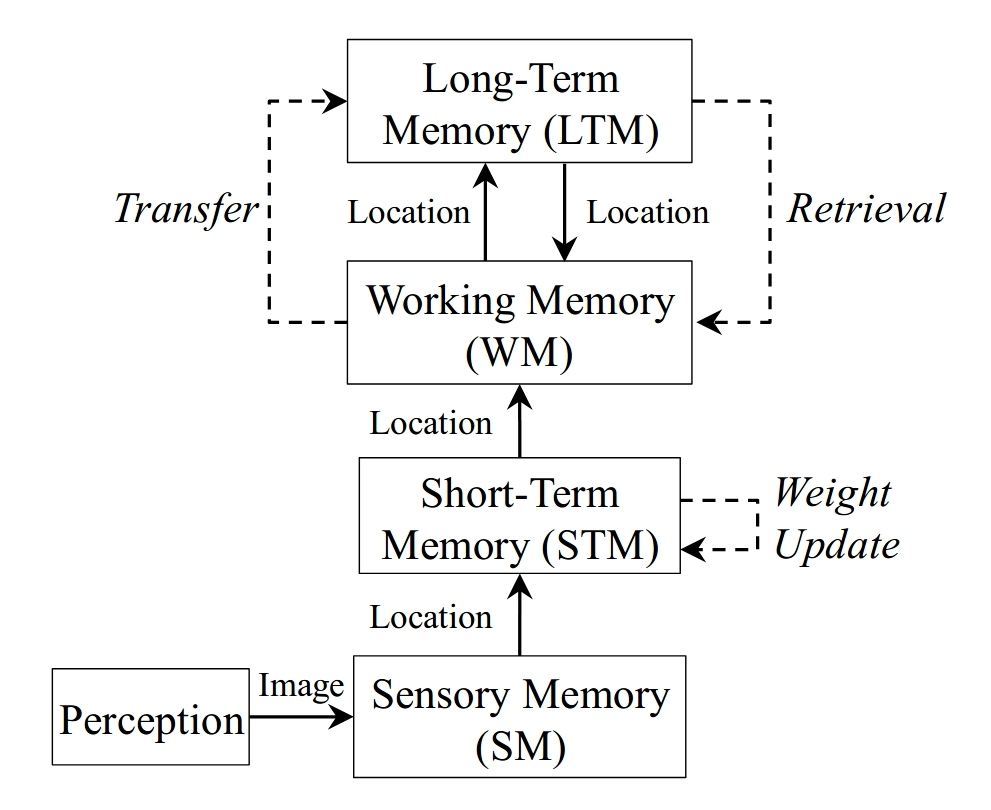
\includegraphics[width=.4\textwidth]{images/rtabmap_memory}
    \caption{Estructura de memoria de la técnica RTAB-Map}
\end{figure}


Se partirá de la premisa de que aquellas localizaciones que son visitadas de forma más frecuente son más propensas a 
crear bucles cerrados. Por ello, el número de veces que una localización sea visitada será empleado como peso, de 
esta forma serán transferidas desde la memoria de trabajo a la memoria de largo plazo aquellas observaciones que 
tengan mayor peso.\\
La memoria a corto plazo, \textit{STM}, tiene como misión buscar las similitudes que existan entre dos imágenes
consecutivas, mientras que la memoria de trabajo, \textit{WM}, es la encargada de detectar los bucles cerrados entre las
localizaciones en el espacio. El número de localizaciones almacenadas en la memoria del trabajo del robot es
limitado. El tamaño de la memoria a corto plazo, \textit{STM}, está basado en la velocidad del robot y en la frecuencia de
adquisición de las localizaciones. \\

% NO SE SI METER ESTA PARTE
\begin{comment}
Es importante destacar que todas las observaciones almacenadas en la memoria a largo plazo, \textit{STM}, del robot no se
usan para detectar bucles cerrados. No obstante, es importante elegir cuidadosamente las localizaciones que se
almacenan en esta memoria. Almacenar las observaciones según la técnica FIFO (First In First Out), sería un
error debido a que, como el algoritmo establece un número máximo de localizaciones que se pueden
almacenar mientras se está explorando un entorno, podríamos alcanzar el superar el umbral de tiempo
establecido sin llegar a cerrar el bucle haciendo que las localizaciones más antiguas nunca consigan asociarse. \\
Como alternativa, el orden de almacenamiento de las observaciones se elige de forma aleatoria, aunque es
preferible mantener en la memoria de trabajo aquellas localizaciones que son más susceptibles de ser
observadas.
\end{comment}
\subsection{Framework de optimización Octomap}
El paquete de ROS empleado para emplear la ténica RTAB-Map,\textit{rtabmap-ros}, posee la posibilidad de extraer también el mapa de ocupación 2D y 3D gracias al Framework 
\textit{Octomap}\footnote{https://octomap.github.io/}. \\
Este framework es una librería de C++ que permite la obtención de mapas probabilisticos basándose en una estructura de representación jerarquica de datos para subdividir
el espacio 3D, esta estructura es denominada \textit{Octotrees}. \\

\begin{figure}[h!]
    \centering
    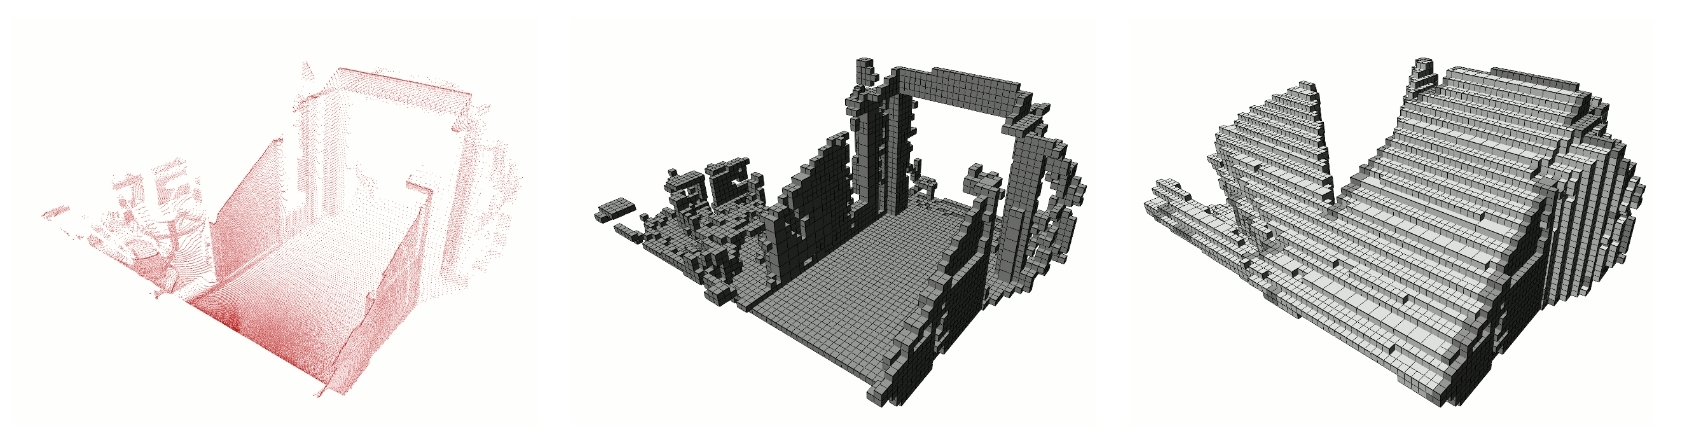
\includegraphics[width=.9\textwidth]{images/octomap_beauty}
    \caption{Optimización realizará empleando los \textit{Octotrees}}
\end{figure}


Los \textit{Octotrees} se emplean para almacenar propiedades booleanas del entorno, en el caso de
la robotica estas propiedas booleanas es la ocupación de dicha celda, de la cual es posible definir su tamaño minimo en función de la resolución de mapa
deseada.
\begin{figure}[h!]
    \centering
    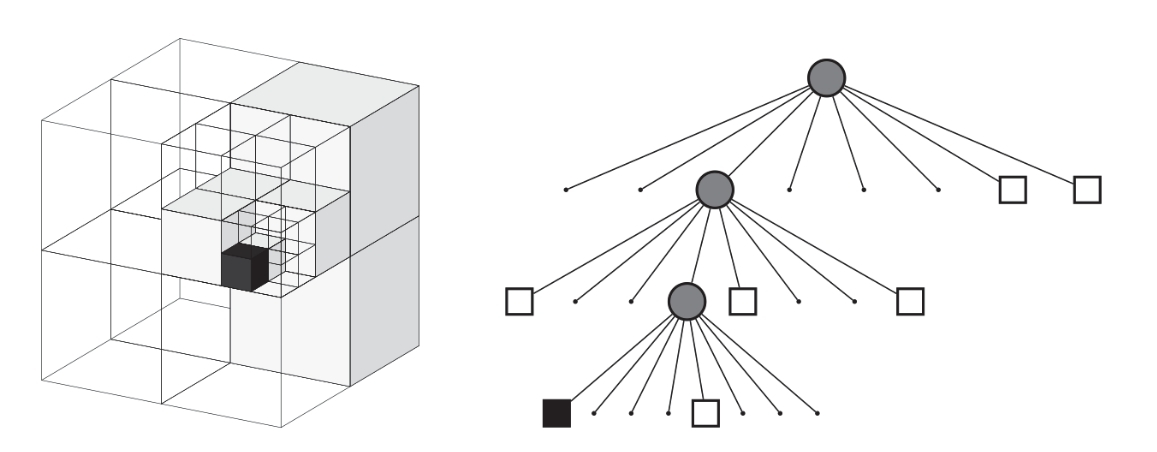
\includegraphics[width=.7\textwidth]{images/octotree}
    \caption{Funcionamiento del \textit{octotree} y su estructura en arbol}
\end{figure}

\newpage
\subsubsection{\textit{ORB-SLAM 2}}
ORB-SLAM2 es una técnica de SLAM en tiempo real para cámaras Monocular, Stereo y RGB-D que se engloba dentro de las técnicas de 
\textit{Sparse-Slam}. Se computa la trayectoria y hace una reconstrucción dispersa 3D del entorno. Al igual que todas las técnicas 
de SLAM, se basa en la detección de bucles cerrados y  se relocaliza en tiempo real. \\
Se basa en la detección de \textit{keyframes} que emplea para hacer un tracking de los mismos y a partir de ello crear el 
mapa local que, posteriormente, se optimizará junto al mapa global. \\
Unos de los puntos destacables de ésta técnica de SLAM son los siguientes:
\begin{itemize}
    \item Emplea \textit{grafo de covisibilidad}. Tanto el seguimiento como el mapping se focalizan en el área covisible,
    independientemente del tamaño del mapa completo, consiguiendo así explorar entornos amplios sin
    aumentar el tiempo y la carga de computación.

    \item La estrategia para detectar los bucles cerrados de visión en tiempo real se basa en la optimización de
   un de grafo denominado \textit{Essencial Graph}, lo cuál se desarrollará mas adelante.
\end{itemize}

A continuación, se tratará un poco el funcionamiento interno del algoritmo, el cuál presenta el siguiente esquema:
\begin{figure}[h!]
    \centering
    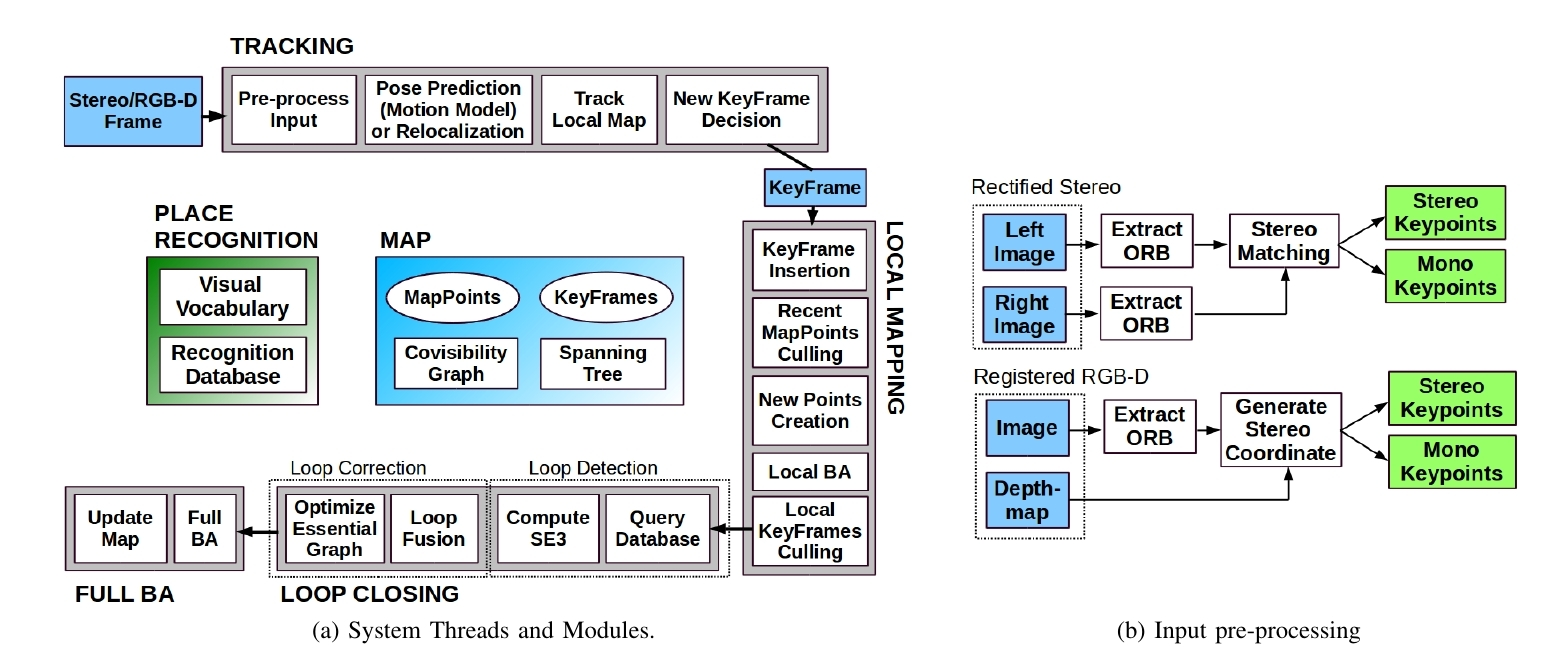
\includegraphics[width=1\textwidth]{images/orb_scheme}
    \caption{Estructura interna de ORB-SLAM2}
\end{figure}

Se observa cómo existen 6 grandes módulos, los cuales de lanzarán en 3 hilos paralelos. \\
En primer lugar, se tendrá el preprocesamiento de la imagen, de la cuál se obtendrán  ORB features 
\textit{(Oriented Fast and Rotated BRIEF)}. \\
Los hilos desempeñarán las siguientes funciones:
\begin{itemize}
    \item El \textit{tracking} se encargará de localizar la cámara en cada frame buscando marches entre las features
    del mapa local y minimizando la reprojección del error aplicando un \textit{Bundle Adjustment}\footnote{https://homes.cs.washington.edu/~sagarwal/bal.pdf} sólo de 
    movimiento.
    \item El \textit{Local Mapping} se encargará de gestionar y optimizar el mapa local aplicando un \textit{BA} local.
    \item El hilo de \textit{Loop Closing} se encargará de detectar bucles cerrados grandes y corregir la deriva acumulada
    realizando una optimización del grafo del \textit{pose} obtenido. Este hilo, lanza 4 hilos internos que se encagarán de
    realizar un \textit{Bundle Adjustement} completo tras la optimización del grafo del \textit{pose}, para hayar la solución
    más optima.
\end{itemize}

En caso de que el sistema pierda el tracking, lleva integrado un modulo de \textit{Plane recognition} basado en un vocabulario 
de palabras que básicamente es una especie de preentrenamiento de la técnica, para poder obtener y asociar keyframes más fácilmente. \\

En la imagen a continuación, puede observarse la técnica corriendo en un ordenador. Destacar que ésta técnica de SLAM presenta una carga computacional bastante elevada.
\begin{figure}[h!]
    \centering
    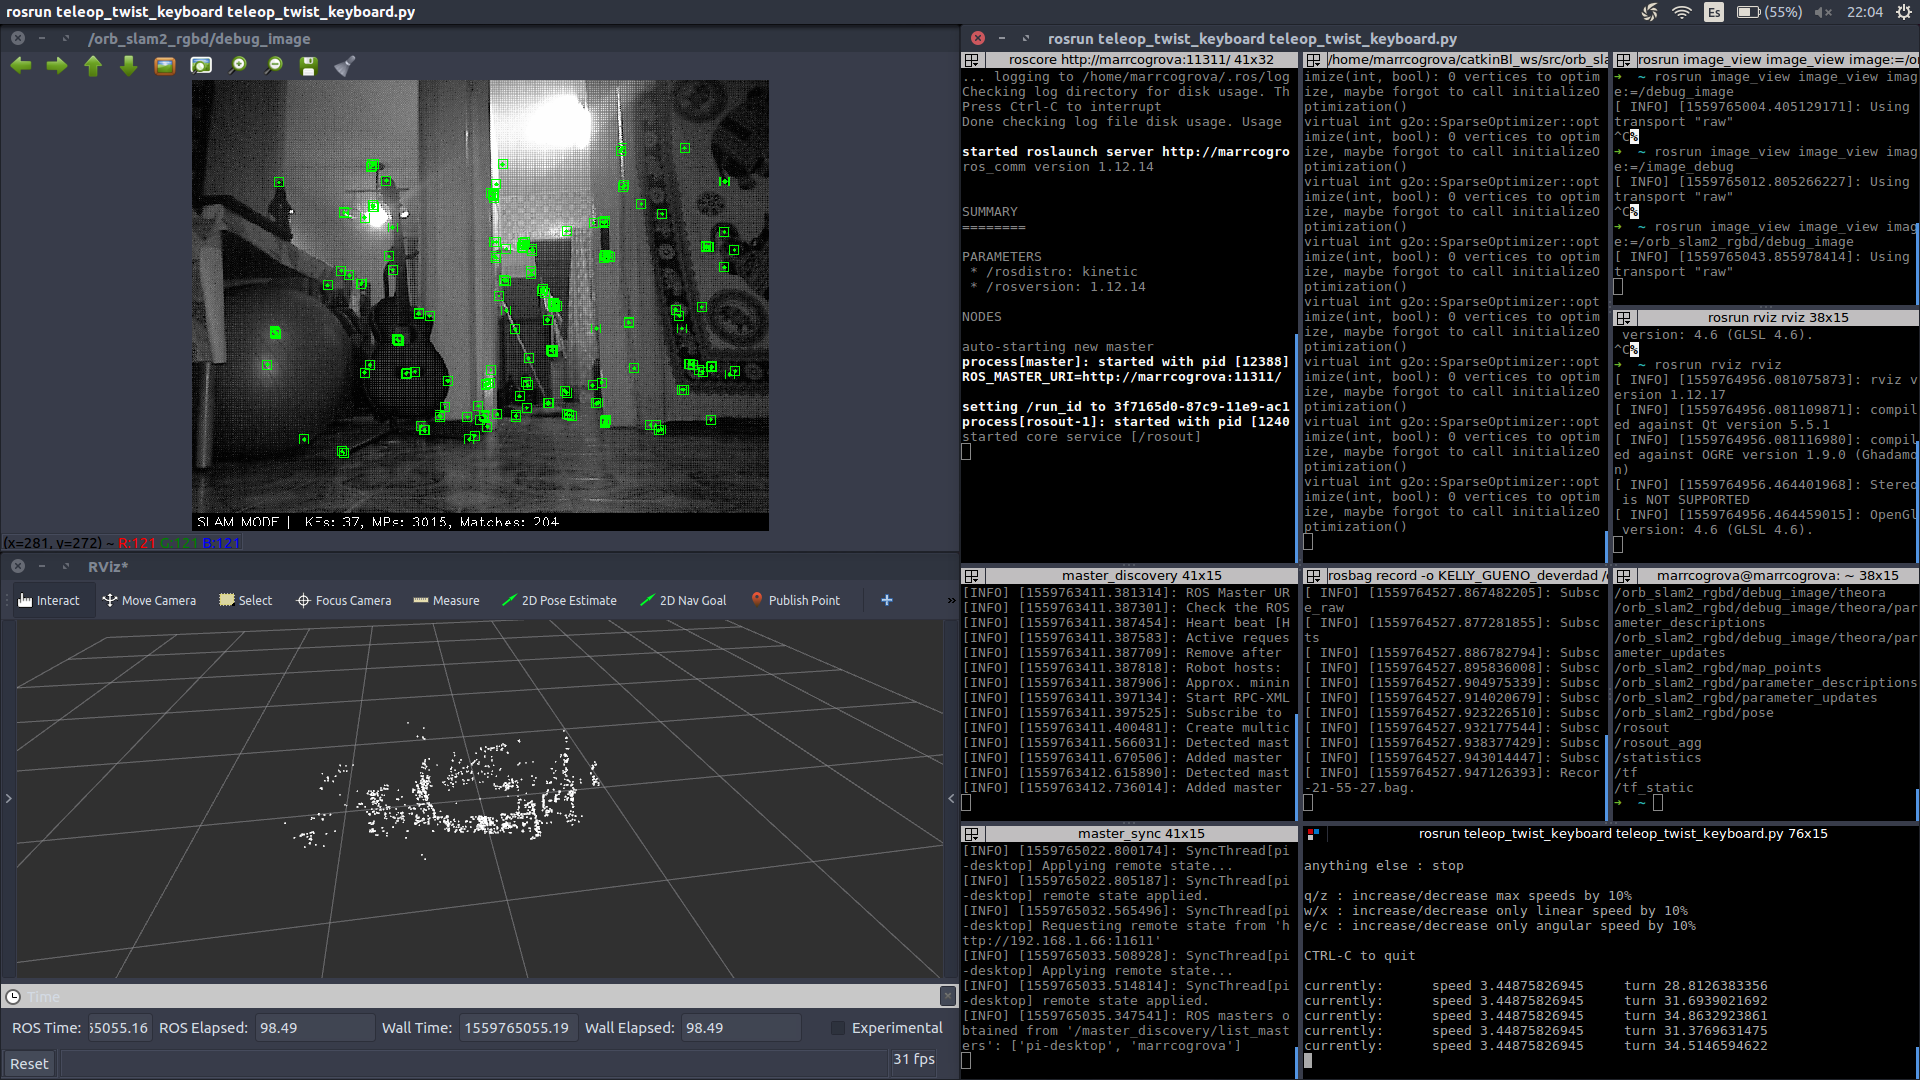
\includegraphics[width=1\textwidth]{images/working_zone_orb}
    \caption{ORB-SLAM2 en funcionamiento}
\end{figure}

Se observa en la imagen superior izquierda las features que está obteniendo en ese frame, a partir de las cuales se ha creado en mapa local y,
por extensión el global. En la imagen inferior izquierda, se puede observar el mapa creado, el cuál se analizará más tarde.\\
Por último, a la derecha se tienen las terminales a partir de las cuales se ha lanzado el SLAM y se realiza la comunicación con el robot.\\

\newpage

\section{Comparativa de resultados empleando \textit{rosbags} del robot}
Para realizar un análisis y una comparativa entre éstas dos técnicas de SLAM, se ha optado por generar un set de datos del robot y correrlo con ambas técnicas,
de tal modo que ambas téngan los mismos datos de entrada y se pueda analizar de mejor modo la salida de la arquitectura. \\
La implementación de todo el sistema, también es posible correrlo en tiempo real con el robot empleando una o la otra técnica, pero de ese modo sería más complejo
realizar una comparativa entre ellas. \\
Estos datasets, que han sido grabados en forma de \textit{rosbag}, se grabaron desde el ordenador en el que corre el SLAM, de todos los topicos que se recibiaN
del ordenador de abordo del robot a través de la comunicación \textit{Multi-master} implementada.\\
A continuación, se muestra una imagen de los topicos contenidos en ambos datasets:
\begin{figure}[h!]
    \centering
    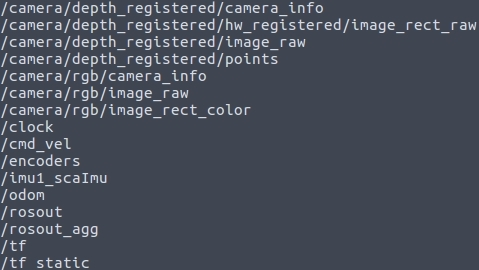
\includegraphics[width=.5\textwidth]{images/topics_bags}
    \caption{topicos contenidos en el bag}
\end{figure}

En ambos datasets el robot recorrerá un camino en torno al salón de la casa de uno de los integrantes del grupo. En el primer dataset, el estado del salón será 
el comun, de modo que haya una parte del mapa que no contendrán muchas features. Sin embargo, en el segundo se colocaron objetos en zonas dónde la cantidad de features
y los contrastes del mapa eran reducidos para así comparar el resultado inicial con uno en un entorno experimental, dónde se ha forzado que el entorno esté lleno de features.\\

Se realizarán 3 pruebas, las cuales se encuentras recogidas en vídeos existentes en la carpeta del proyecto. En primer lugar se mostrará el mapa creado por \textit{RTAB-Map} y
la estimación del \textit{path} del robot. Tras ello, se mostrará el mapa de ocupación generado por \textit{OctoMap} tanto en 2D cómo en 3D y, por último, se mostrará el
resultado obtenido con \textit{ORB-SLAM2 RGB-D}.
\newpage

\subsection{Análisis de resultados con el primer \textit{rosbag}}
Este dataset será el que contiene el salón en un estado común, sin alterar la cantidad de features existentes en el entorno. \\
En él, se recorrerá un camino de, aproximadamente, 1$m^2$ en torno al salón.

\subsubsection{RTAB-Map y local path}
En primer lugar, se mostrará el mapa denso obtenido gracias a RTABMAP. Se obsrrva cómo, el loop closure del mapa ha funcionado correctamente de tal modo que la estructura final
del mapa será el rectangulo que confirma el salón.
\begin{figure}[h!]
    \centering
    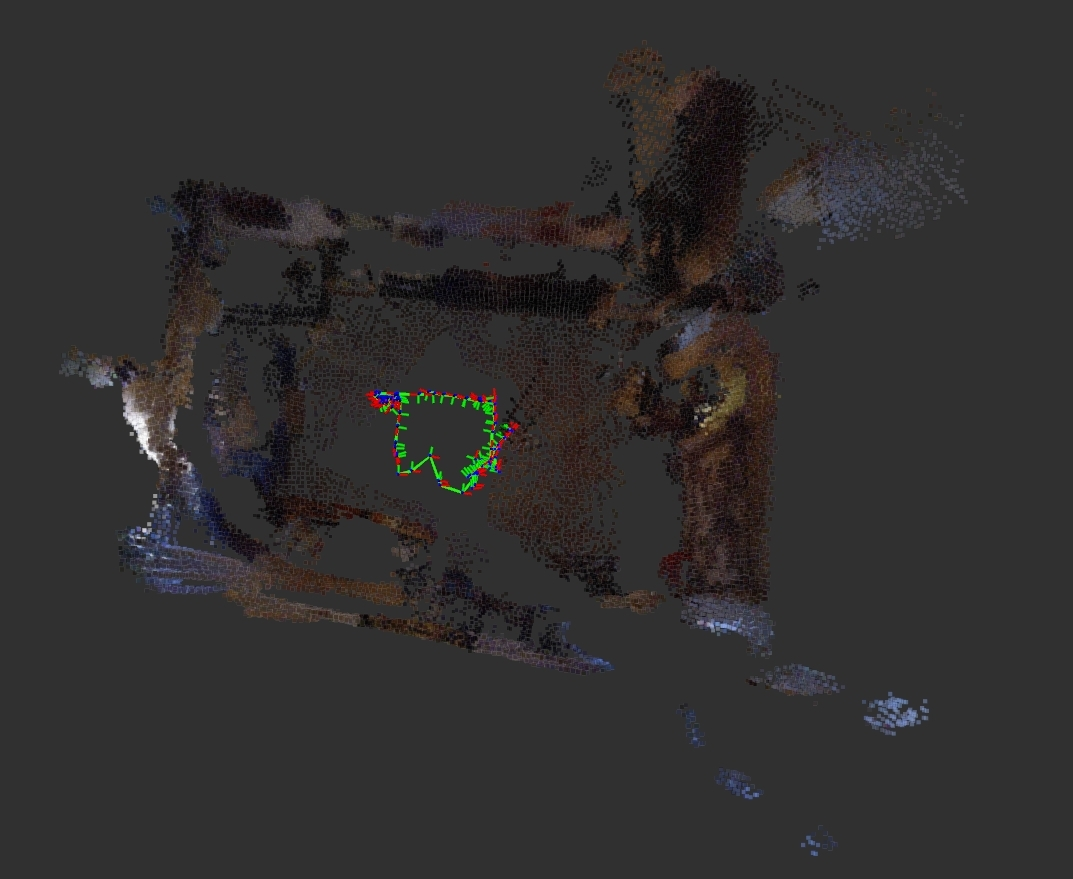
\includegraphics[width=.4\textwidth]{images/slam/bag1_rtabmap_noLC}
    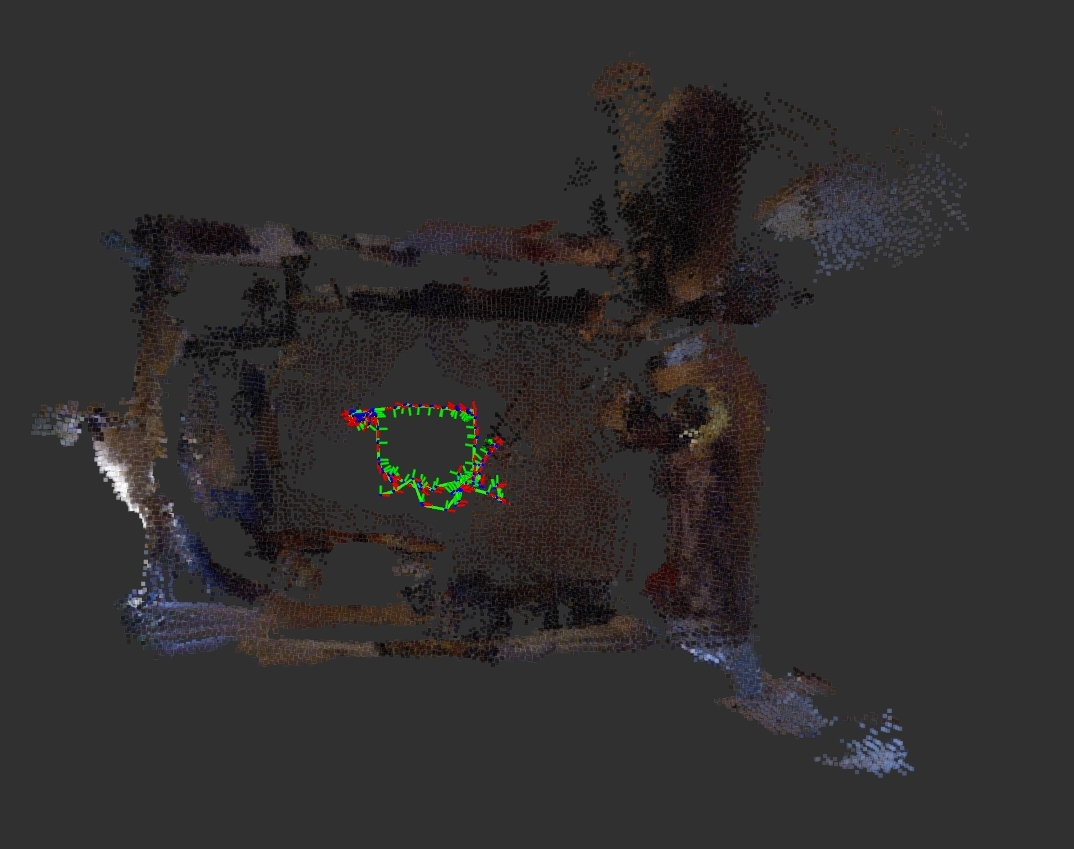
\includegraphics[width=.415\textwidth]{images/slam/bag1_rtabmap_LC}
    \caption{Mapa creado antes y después del \textit{Loop Closure}}
\end{figure}

El mapa obtenido, será un mapa denso el cual posee toda la información posible del entorno, cómo se muestra a continuación:
\begin{figure}[h!]
    \centering
    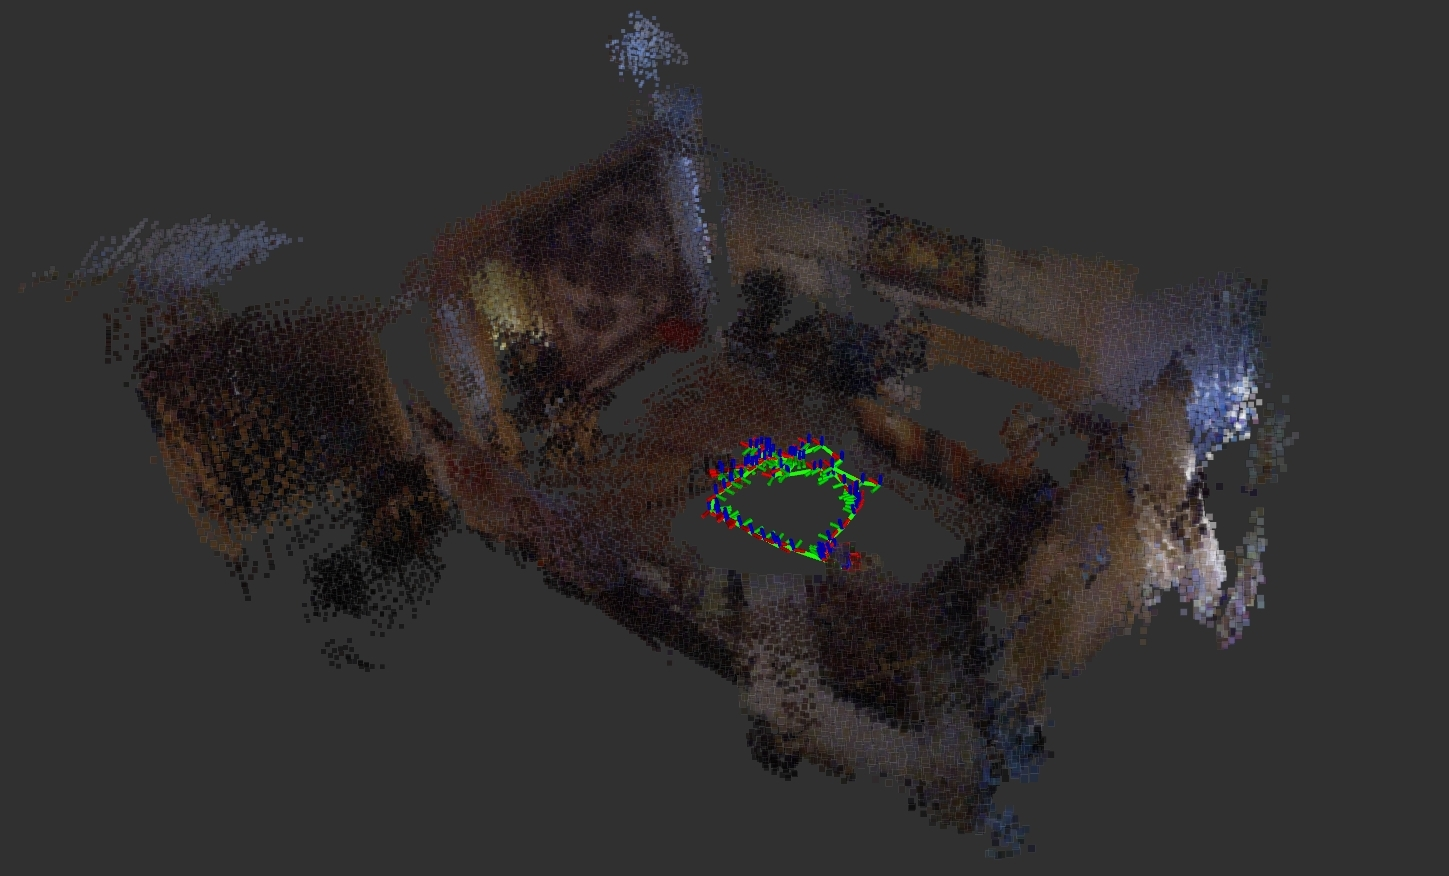
\includegraphics[width=.9\textwidth]{images/slam/bag1_rtabmapbonito}
    \caption{Mapa obtenido con RTAB-Map}
\end{figure}

Gracias a la realización de dicho mapa, se ha optado por medir la tela grande de la pared y el cuadro sobre el sillón naranja tanto en el mapa cómo la distancia real, para comprobar
el error que posee ésta técnica.

\begin{center}
\begin{tabular}{ c | c | c | c }
     & Ancho en el mapa creado & Ancho real & Error de RTAB-Map\\
     \hline
     Tela de la pared & 1.75 m & 2 m & 0.15m\\
     Cuadro sobre sillón & X cm & X cm \\
\end{tabular}
\end{center}

En este caso, se obsrrva que ...

\subsubsection{OctoMap}
Gracias a \textit{Octomap} se ha obtenido el mapa de ocupación probabilistico del entorno. Se mostrará, al igual que antes, el mapa antes y despues del loop closure, ya que es local
destacable de ésta técnica de SLAM.
\begin{figure}[h!]
    \centering
    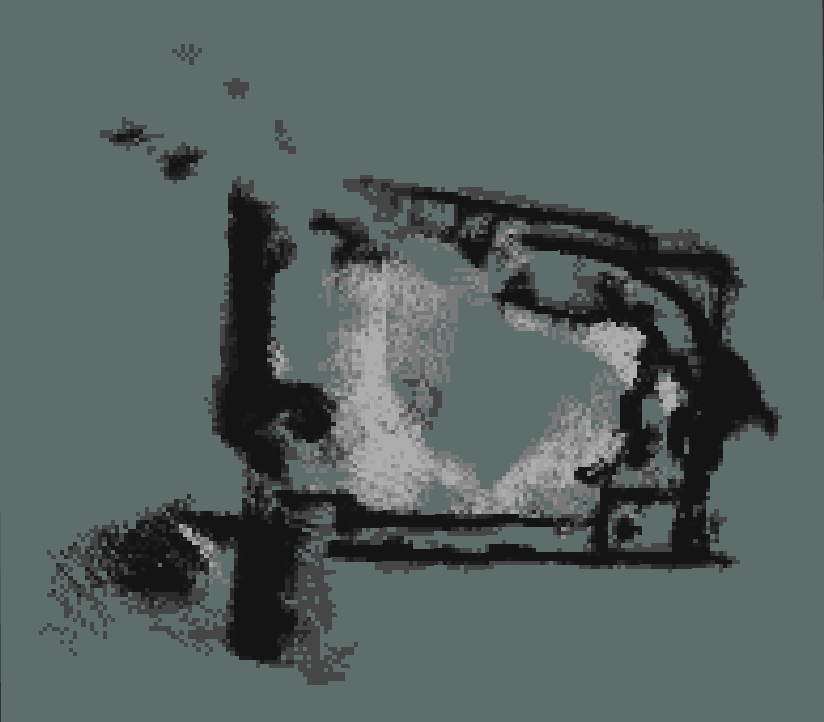
\includegraphics[width=.4\textwidth]{images/slam/bag1_occupGrid_noLC}
    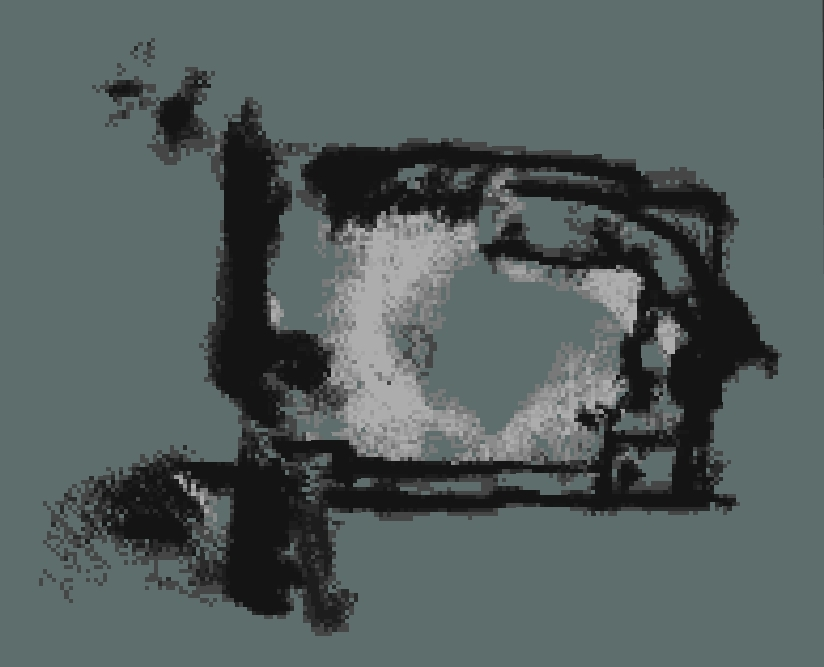
\includegraphics[width=.435\textwidth]{images/slam/bag1_occupGrid_LC}
    \caption{Mapa de ocupación antes y despues del \textit{Loop Closure}}
\end{figure}

Además, \textit{Octomap} nos proporciona el mapa de ocupación 3D, cómo el mostrado a continuación:
\begin{figure}[h!]
    \centering
    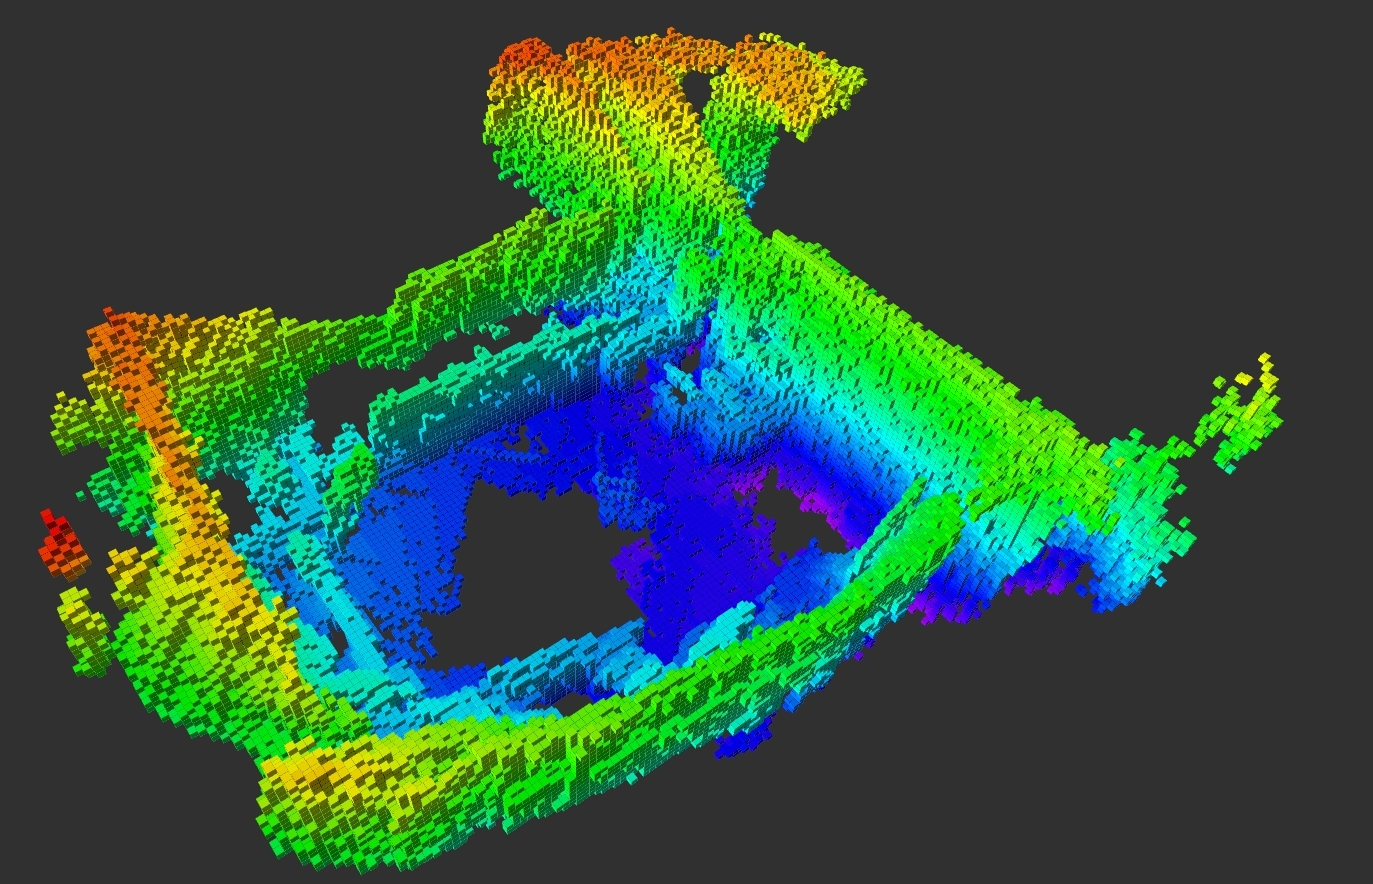
\includegraphics[width=.9\textwidth]{images/slam/bag1_octomap_LC}
    \caption{Mapa obtenido con RTAB-Map y empleando el framework \textit{Octomap}}
\end{figure}

\subsubsection{ORB-SLAM2 RGB-D}
En el caso del ORB-SLAM2, con éste dataset los resultados han sido peores, debido a que en cierto momento, los cambios de iluminosidad procedentes del balcón de la casa, hacen que se
se pierda dentro del mapa creado. A continuación se muestra el frame anterior a la pérdida de la localización dentro del mapa. Los colores representan la altura en el eje Z.
\begin{figure}[h!]
    \centering
    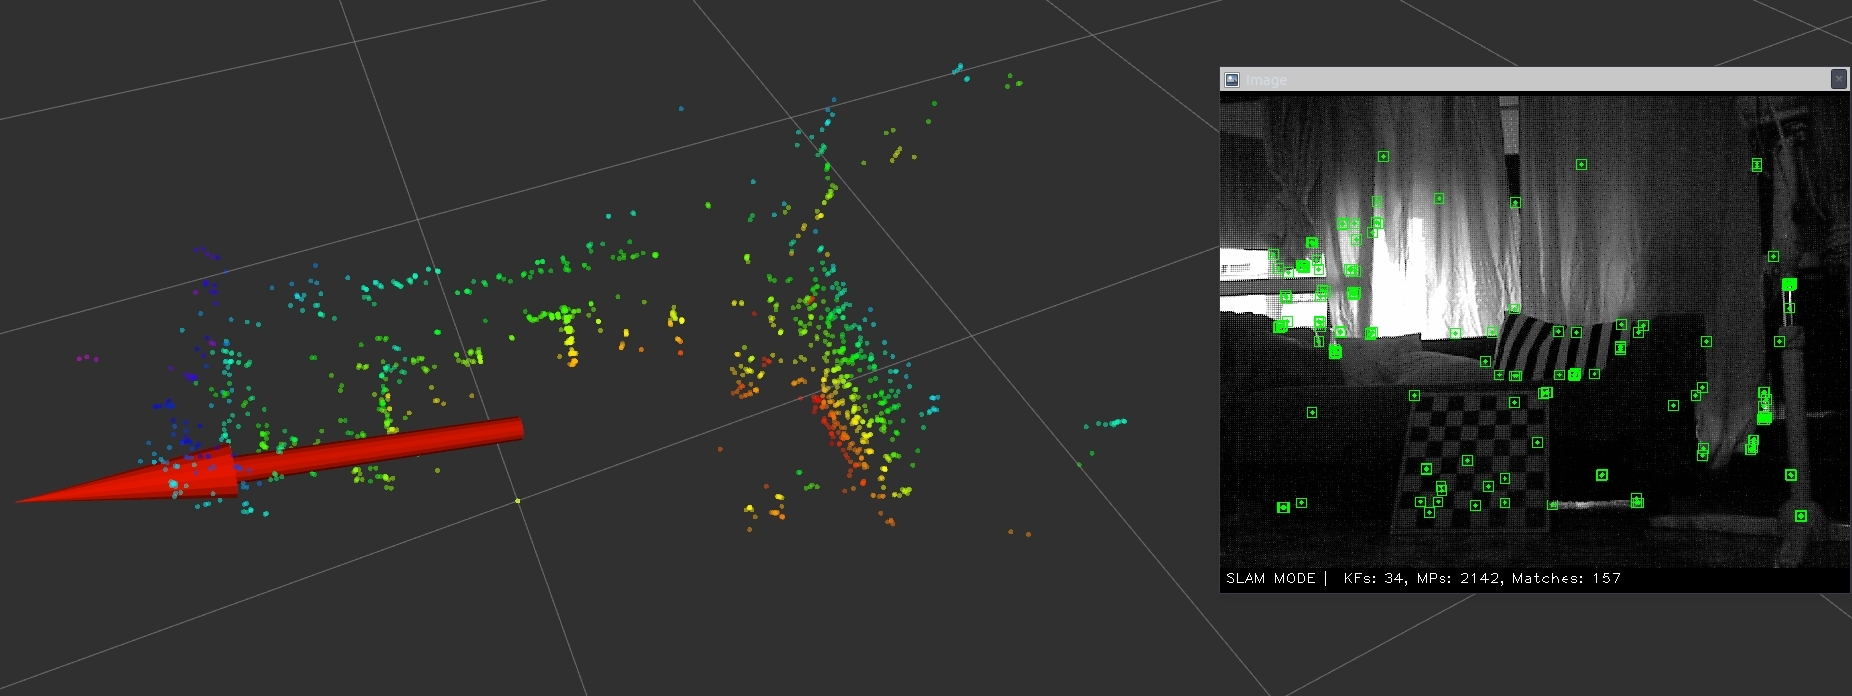
\includegraphics[width=.9\textwidth]{images/slam/bag1_orb_beforeLOSE}
    \caption{Momento anterior a la pérdida del robot en el primer dataset}
\end{figure}

Sin embargo, se observa cómo, cuándo vuelve a ver el inicio del mapa, dónde tomó un número elevado de features, se relocalizará, cómo se muestra a continuación:
\begin{figure}[h!]
    \centering
    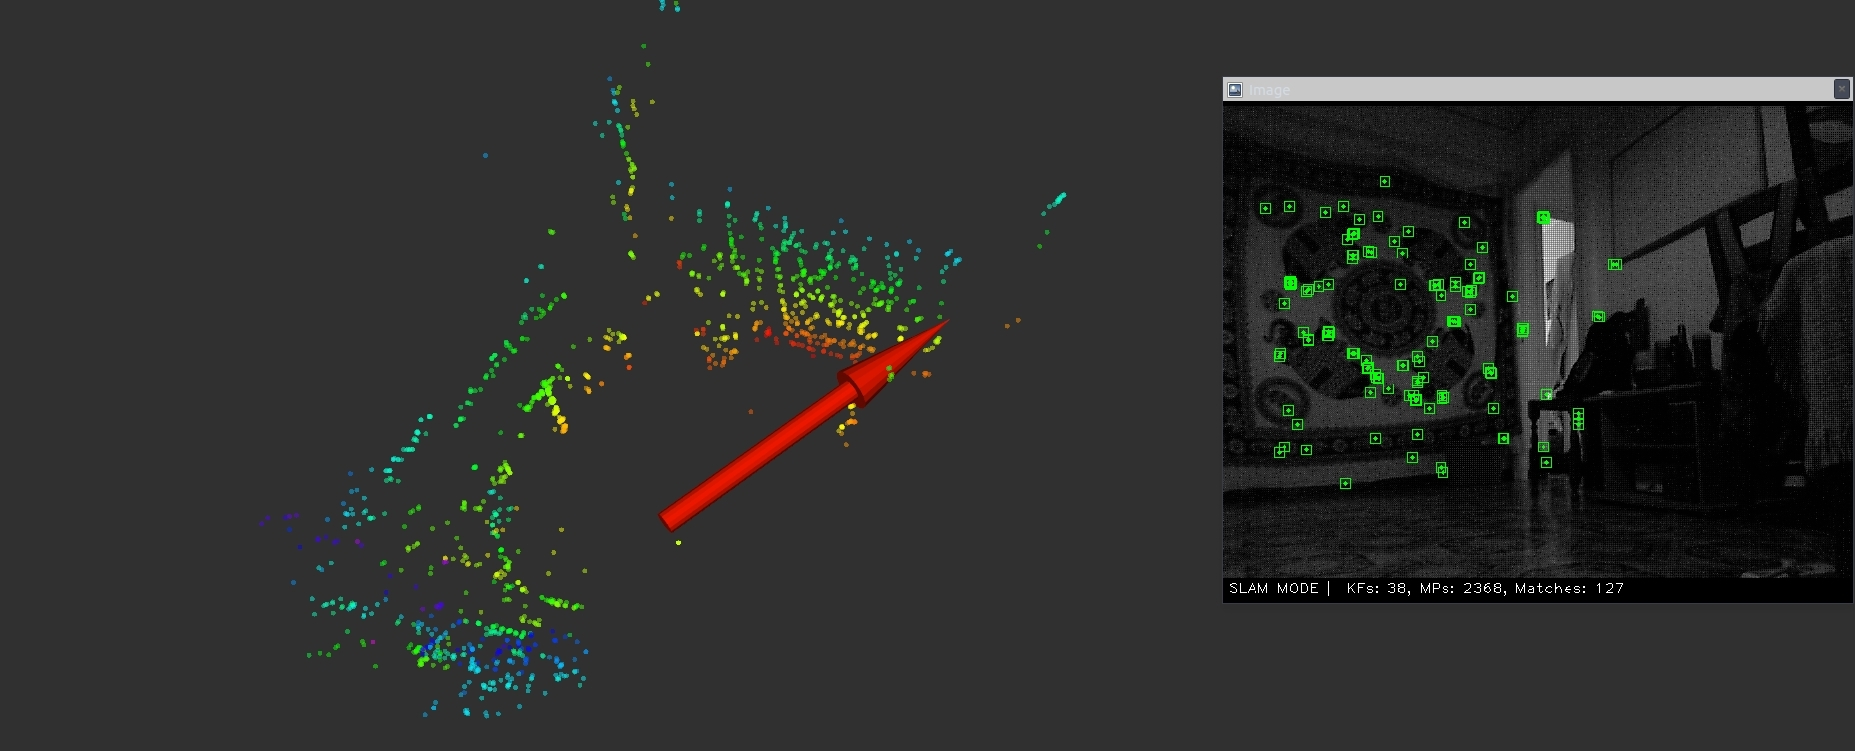
\includegraphics[width=.9\textwidth]{images/slam/bag1_orb_relocal}
    \caption{Relocalización del robot en el primer dataset}
\end{figure}

Debido a que el mapa no se ha llegado a completar se ha obtado por no realizar una comparativa de las medidas en éste caso.

\newpage

\subsection{Análisis de resultados con el segundo \textit{rosbag}}
En éste segundo dataset, el escenario será más parecido a un escenario experimental debido a que se han colocado objetos por el salón de tal modo que en todo el mapa se
obtengan una cantidad elevada de features.

\subsubsection{RTAB-Map y local path}
Al igual que anteriormente, se destacará el loop closure detectado por el mapa. Se observa cómo, antes de dicho momento, las imagenes de la tela de la pared aparecen superpuestas,
sin embargo, posteriormente, se observa cómo ha detectado que ya conocia ese setpoint y cerró el bucle:
\begin{figure}[h!]
    \centering
    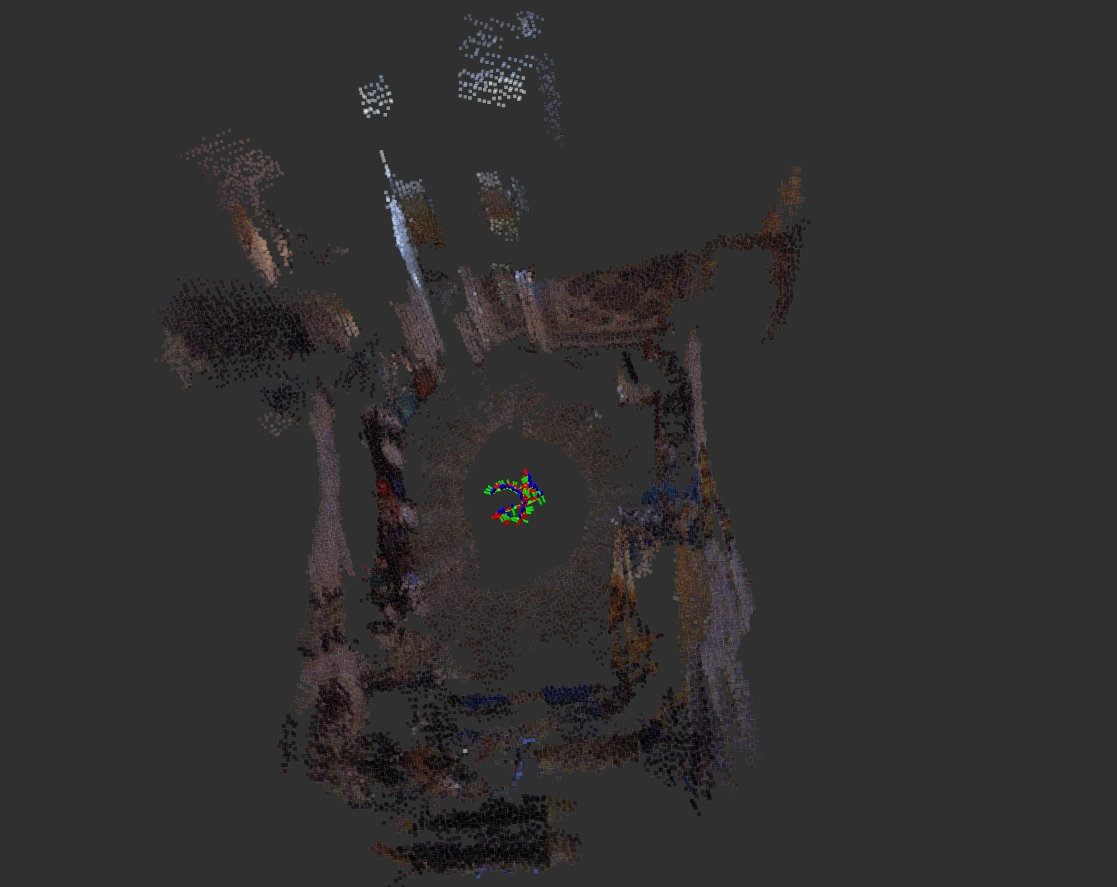
\includegraphics[width=.4\textwidth]{images/slam/bag3_rtabmap_noLC}
    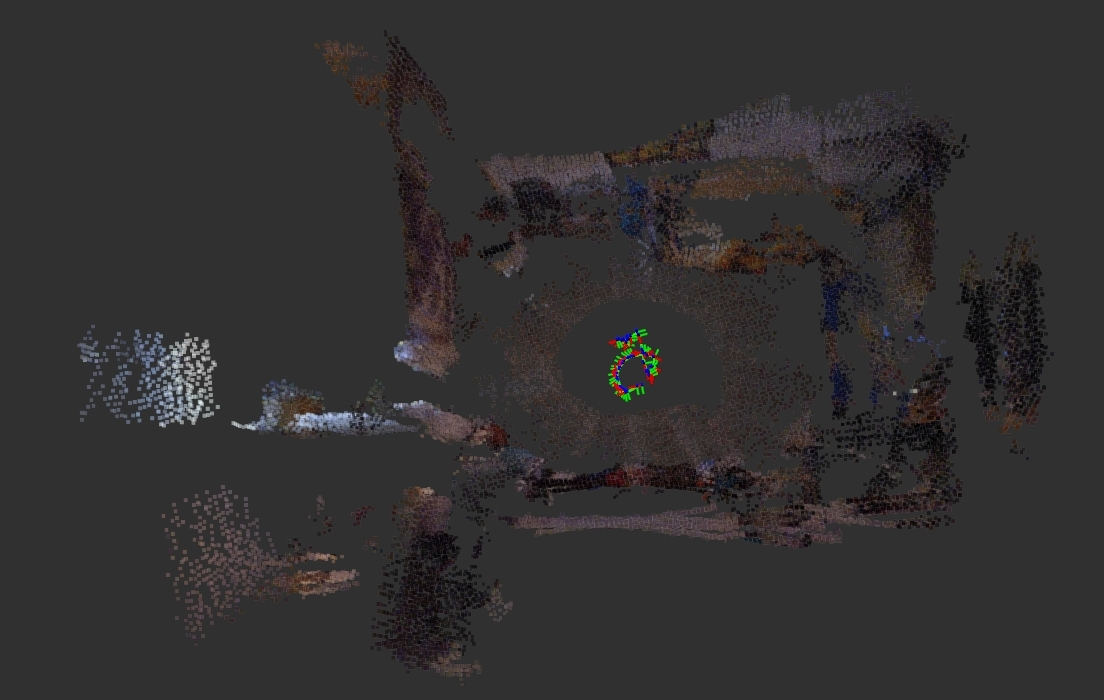
\includegraphics[width=.51\textwidth]{images/slam/bag3_rtabmap_LC}
    \caption{Mapa creado antes y después del \textit{Loop Closure} con el segundo dataset}
\end{figure}

El mapa obtenido, será un mapa denso el cual posee toda la información posible del entorno, cómo se muestra a continuación:

\begin{figure}[h!]
    \centering
    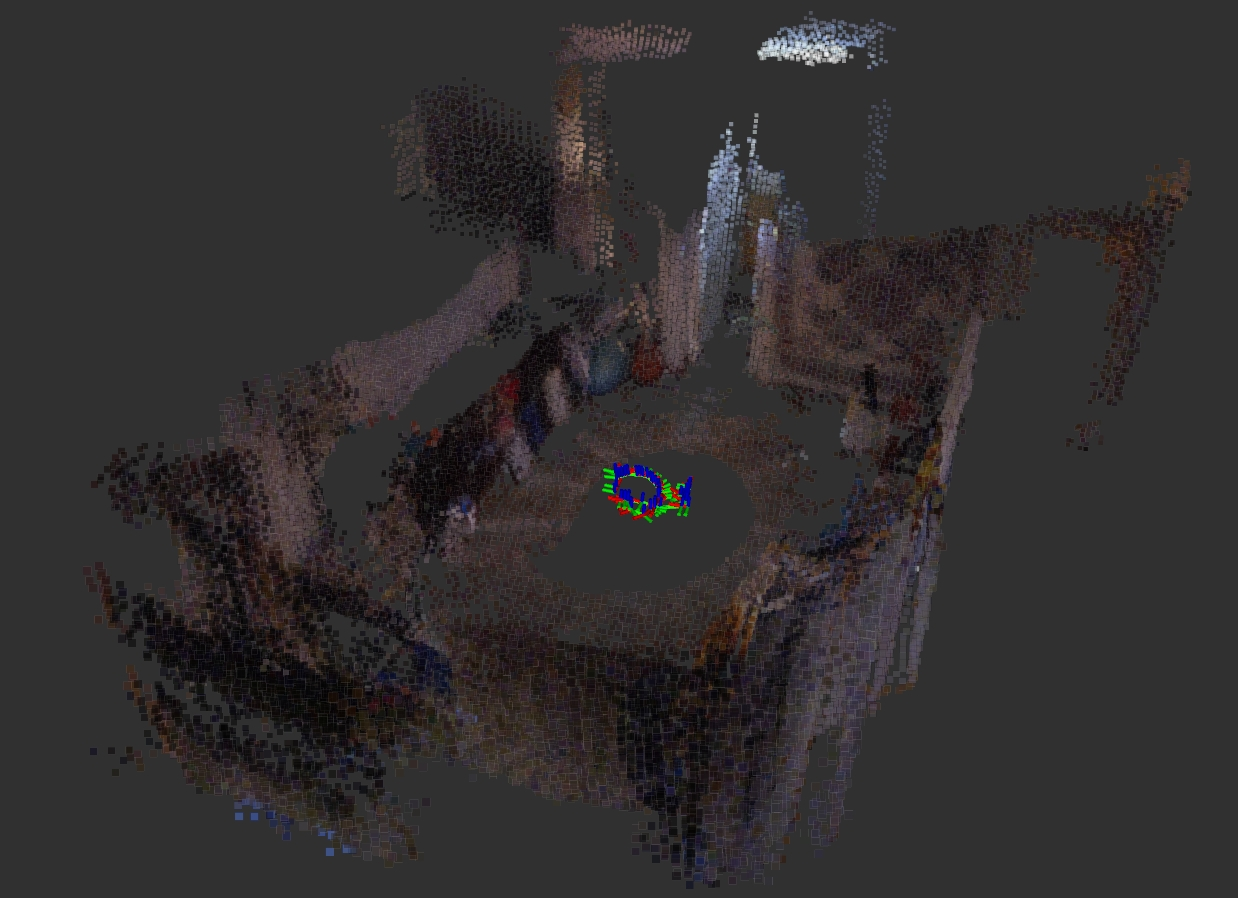
\includegraphics[width=.7\textwidth]{images/slam/bag3_rtabmapbonito}
    \caption{Mapa obtenido con RTAB-Map empleando el segundo dataset}
\end{figure}
    
    \subsubsection{OctoMap}
Gracias a \textit{Octomap} se ha obtenido el mapa de ocupación probabilistico del entorno. Se mostrará, al igual que antes, el mapa antes y despues del loop closure, ya que es local
destacable de ésta técnica de SLAM.
\begin{figure}[h!]
    \centering
    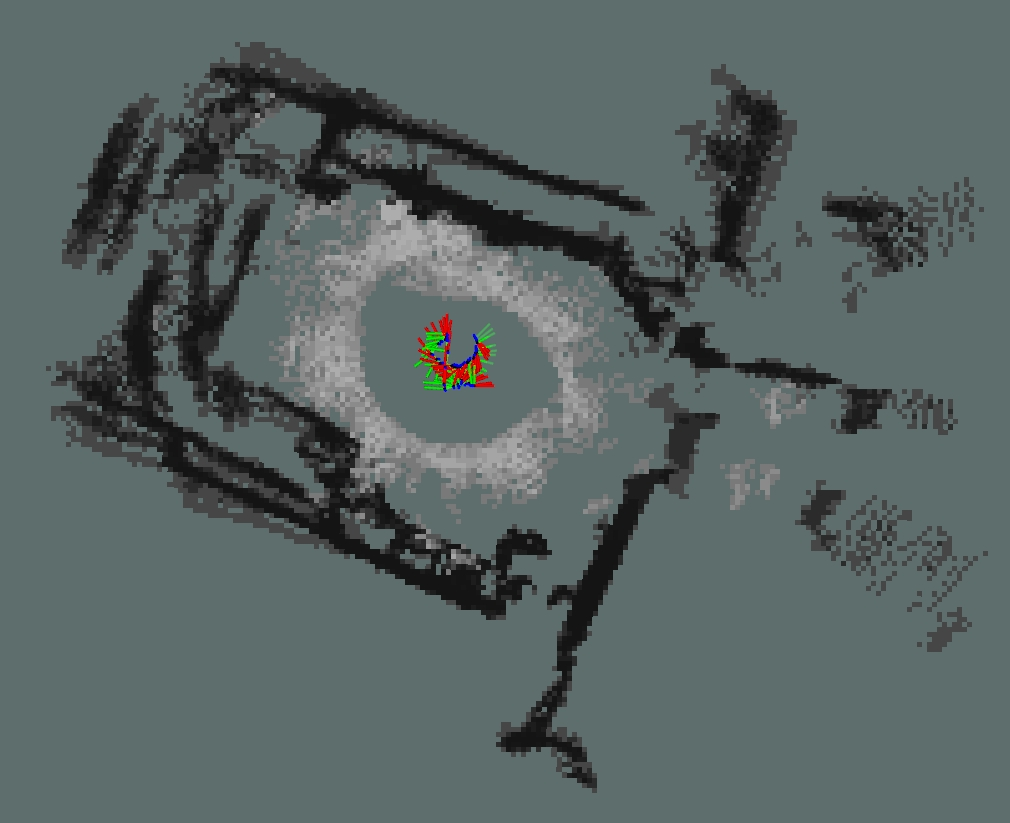
\includegraphics[width=.4\textwidth]{images/slam/bag3_occupGrid_noLC}
    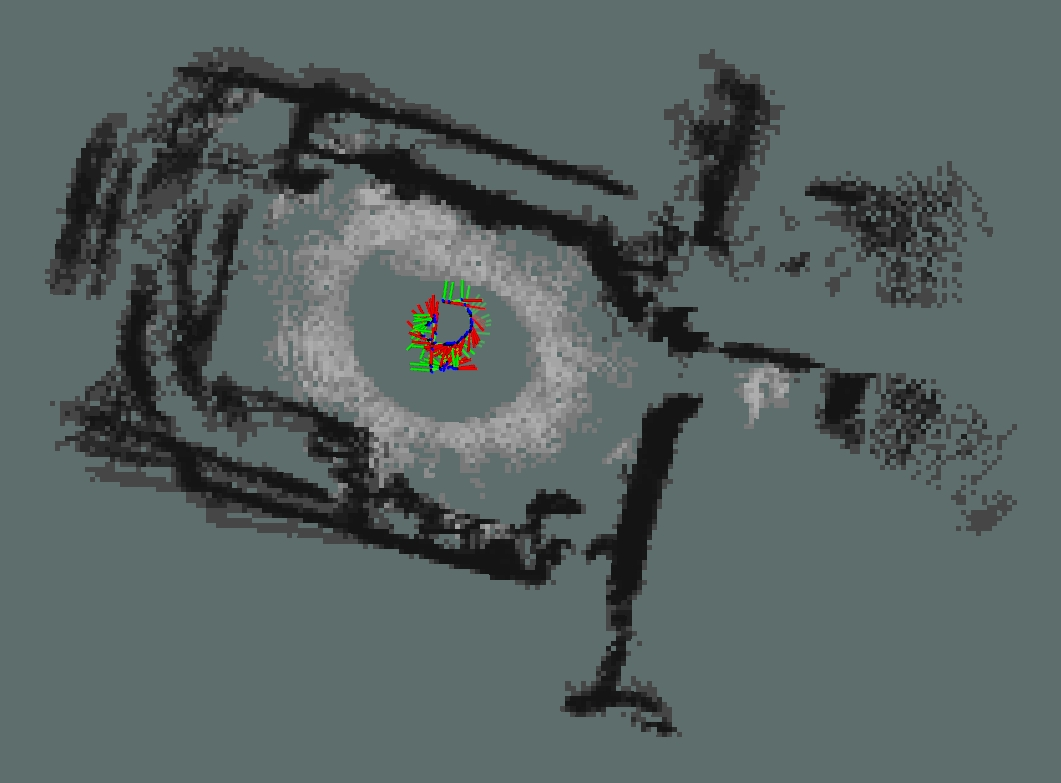
\includegraphics[width=.435\textwidth]{images/slam/bag3_occupGrid_LC}
    \caption{Mapa de ocupación antes y despues del \textit{Loop Closure}}
\end{figure}

Además, \textit{Octomap} nos proporciona el mapa de ocupación 3D, cómo el mostrado a continuación:
\begin{figure}[h!]
    \centering
    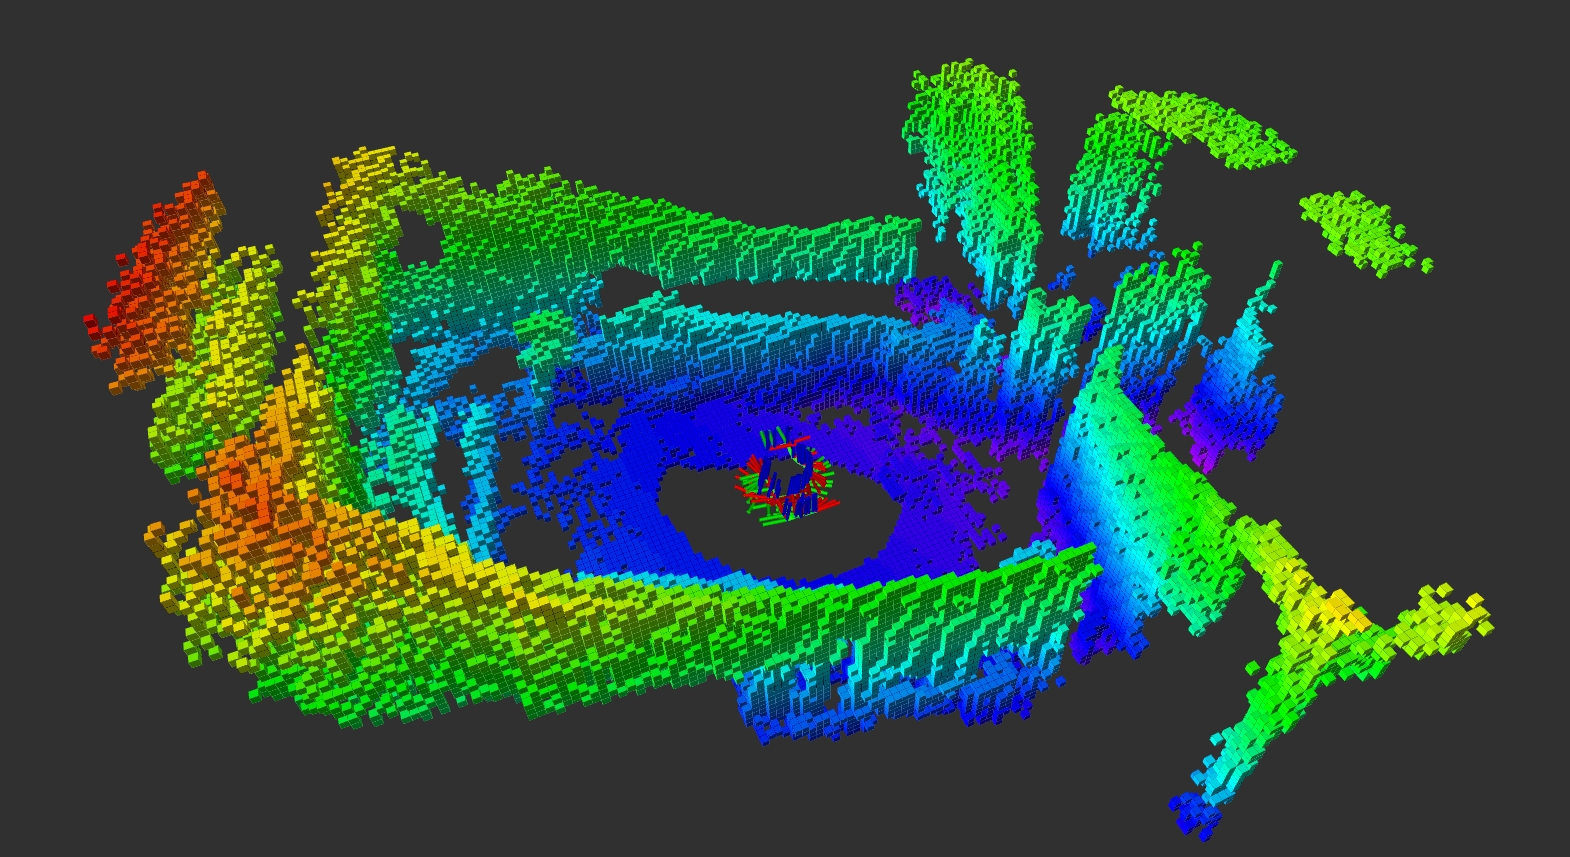
\includegraphics[width=.9\textwidth]{images/slam/bag3_octomap_LC}
    \caption{Mapa obtenido con RTAB-Map y empleando el framework \textit{Octomap}}
\end{figure}

\newpage
\subsubsection{ORB-SLAM2 RGB-D}
En éste segundo set de datos, se evitó el cambio de iluminación en el punto dónde antes se perdio, de tal modo que en éste caso no pase y, efectivamente, cómo se mostrará a continuación,
en ese punto no se perdió:
\begin{figure}[h!]
    \centering
    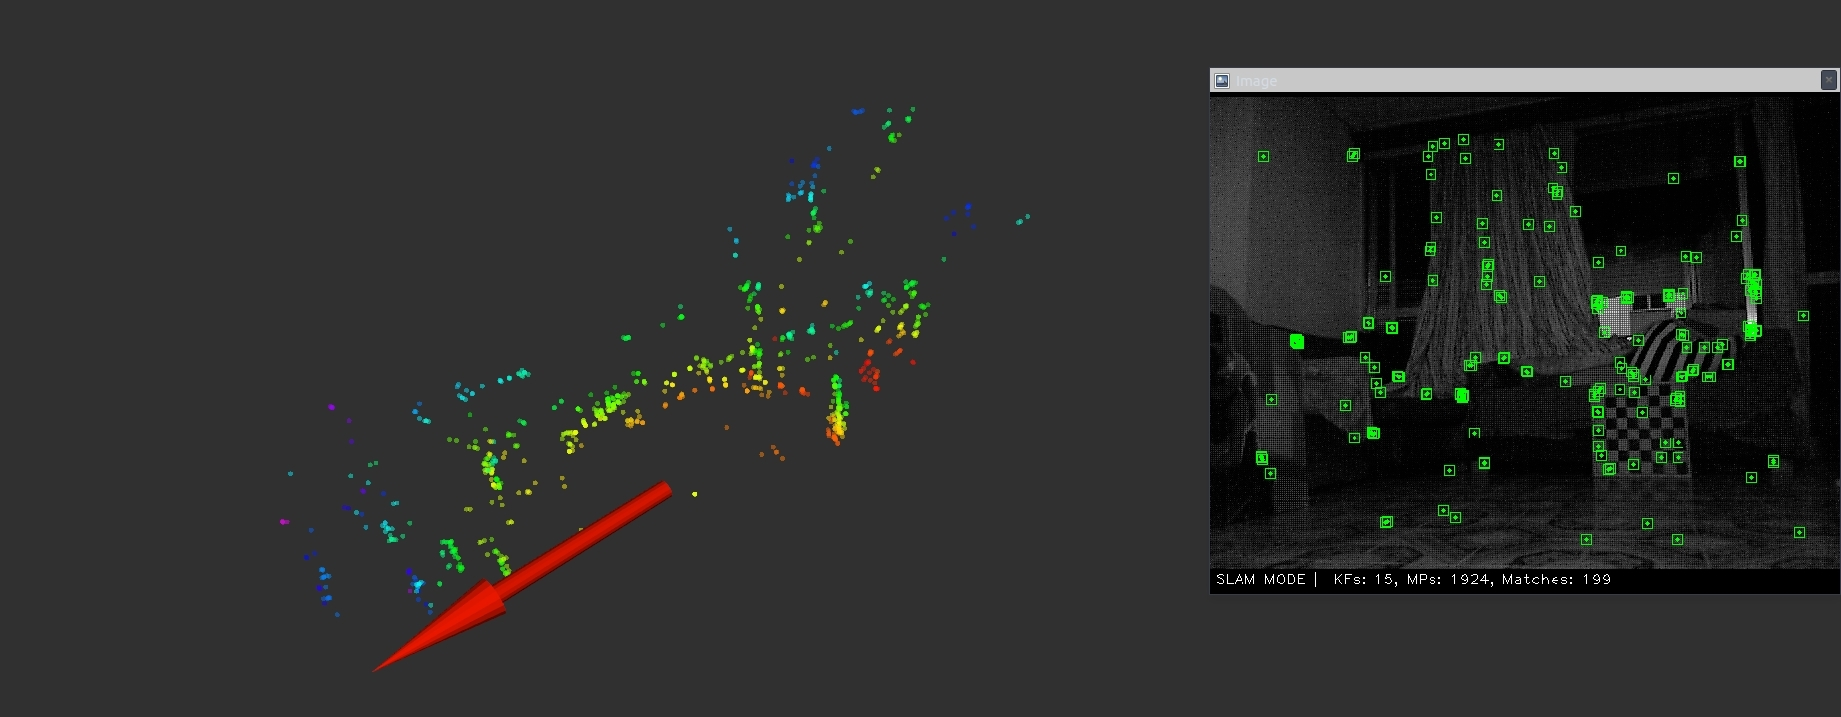
\includegraphics[width=.9\textwidth]{images/slam/bag3_orb_avoidLOSE}
    \caption{Modificación del entorno para evitar la perdida de ORB}
\end{figure}

Por tanto, en éste caso sí se ha logrado obtener un mapa disperso del entorno:
\begin{figure}[h!]
    \centering
    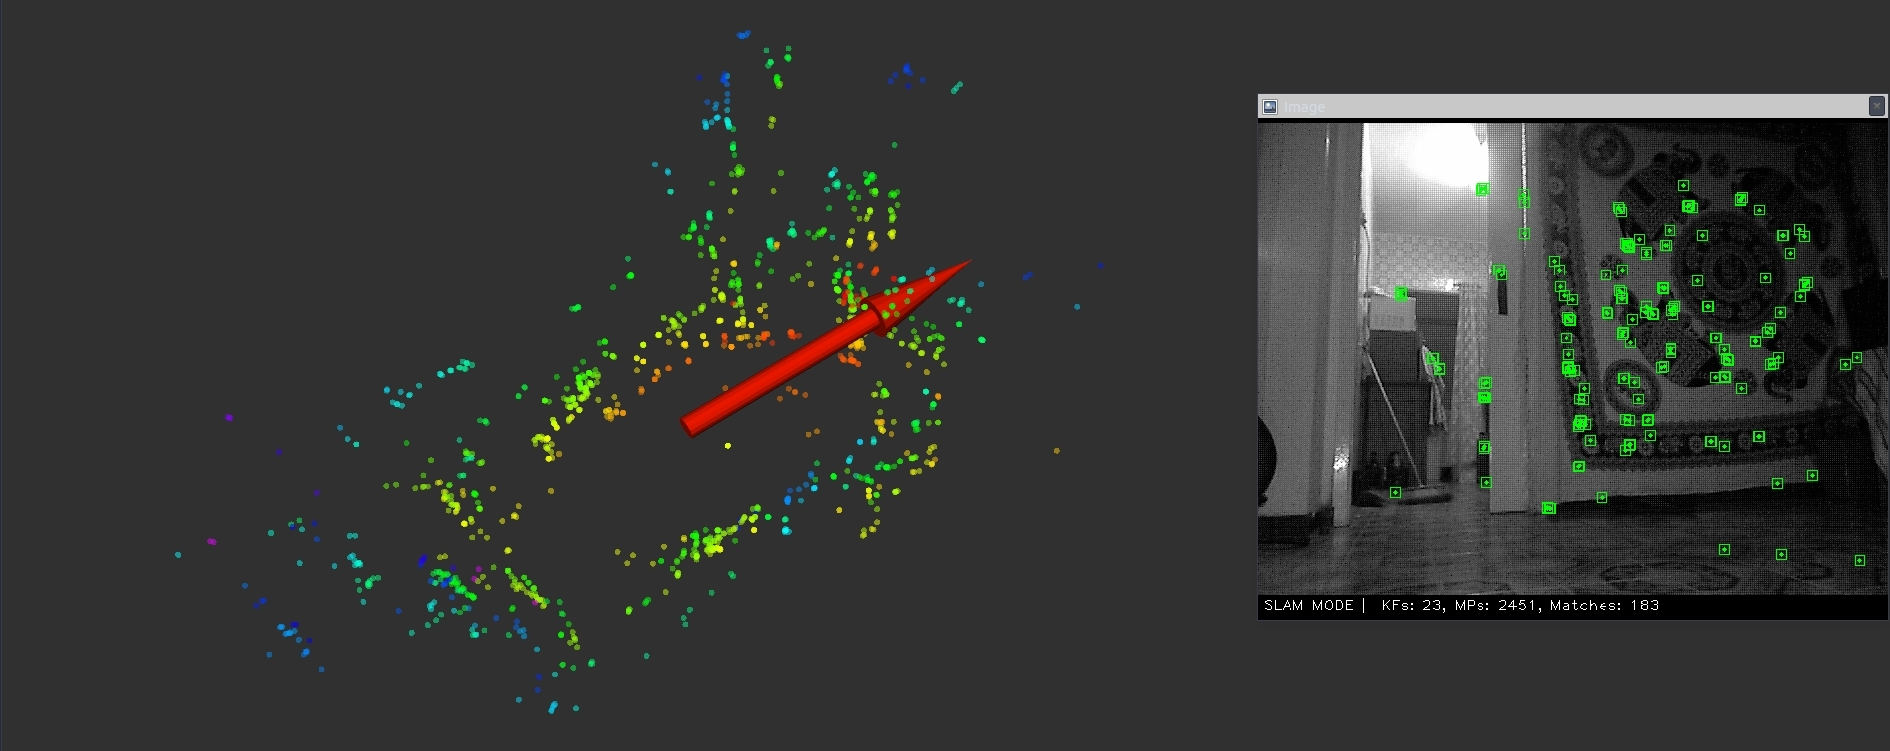
\includegraphics[width=.9\textwidth]{images/slam/bag3_orb_map}
    \caption{Mapa del entorno empleando ORB-SLAM2}
\end{figure}

\newpage
\subsection{Resultados obtenidos de ORB-SLAM2 Monocular}
Debido a la compleja inicialización que conlleva emplear ésta técnica monocular, no ha sido posible evaluar su funcionamiento con los bags generados, ya que no se logró que se
inicializase. Sin embargo, para comprobar su funcionamiento, se ha optado por mover la cámara \textit{Hand-handle}, de tal modo que se asegure la inicialización del SLAM. \\
El gran punto a favor que posee el empleo de SLAM monocular es que no es sensible a la luz, de tal modo que funciona correctamente en exteriores. \\
Por ello, la prueba realiza es en el mismo salón, pero saliendo al balcón y grabando al exterior. \\


\newpage
\bibliography{orb_cite}
\nocite{murORB2}
\nocite{rtabmap}
\nocite{MooreStouchKeneralizedEkf2014}
\nocite{PyCmdMessenger}
\nocite{CmdMessenger}
\nocite{WinNT}
\nocite{atmega}
% \url{http://introlab.github.io/rtabmap/} \\
% \url{https://introlab.3it.usherbrooke.ca/mediawiki-introlab/images/7/7a/Labbe18JFR_preprint.pdf} \\
% \url{https://introlab.3it.usherbrooke.ca/mediawiki-introlab/images/b/bc/TRO2013.pdf}
\end{document}